\documentclass[12pt]{article}
\usepackage{tempora}
\usepackage[utf8]{inputenc}
\usepackage[T2A]{fontenc}
\usepackage{cmap}
\usepackage{mathtext}
\usepackage{array}
\usepackage{booktabs}
\usepackage{multirow}
\usepackage[russian,english]{babel}

\usepackage{amsmath,amsfonts,amssymb,amsthm,mathtools} % AMS
\usepackage{icomma}

\usepackage[left=10mm, top=20mm, right=18mm, bottom=15mm, footskip=10mm]{geometry}
\usepackage{indentfirst}
\usepackage{euscript}	 % Шрифт Евклид
\usepackage{mathrsfs} % Красивый матшрифт

\usepackage[italicdiff]{physics}
\usepackage{graphicx}
\graphicspath{{images/}}
\DeclareGraphicsExtensions{.pdf,.png,.jpg}
\usepackage{wrapfig}
\usepackage{subcaption}
\usepackage{caption}
\usepackage{hyperref}
\usepackage[rgb]{xcolor}



\hypersetup{				% Гиперссылки
    colorlinks=true,       	% false: ссылки в рамках
	urlcolor=blue          % на URL
}
\captionsetup[figure]{name=Рисунок}
\captionsetup[table]{name=Таблица}


% Определяем команду для строки оглавления с отточками
\newcommand{\tocline}[2]{%
  \noindent\makebox[0pt][l]{#1}\hfill
  \leaders\hbox to 1.5mm{\hss.\hss}\hfill
  \makebox[0pt][r]{#2}\par
}

% Альтернативный стиль (более надёжный, работает всегда):
\newcommand{\tocentry}[2]{%
  \noindent
  \parbox[t]{0.8\textwidth}{\raggedright #1}%
  \parbox[t]{0.15\textwidth}{\raggedleft #2}%
  \par
  \vspace{-1.2\baselineskip}
  \noindent\leaders\hbox to 1.5mm{\hss.\hss}\hfill\mbox{}%
  \par
  \vspace{0.8\baselineskip}
}

% Но самый простой и надёжный способ — через \dotfill:
\newcommand{\tocitem}[2]{%
  \noindent #1 \dotfill\ #2\par
}


\begin{document}

\thispagestyle{empty}

\begin{center}

% Верхняя часть титульного листа
\large
Министерство науки и высшего образования Российской Федерации \\
\large
ФЕДЕРАЛЬНОЕ ГОСУДАРСТВЕННОЕ АВТОНОМНОЕ \\
ОБРАЗОВАТЕЛЬНОЕ УЧРЕЖДЕНИЕ ВЫСШЕГО ОБРАЗОВАНИЯ \\
\large
«МОСКОВСКИЙ ФИЗИКО-ТЕХНИЧЕСКИЙ ИНСТИТУТ \\
(НАЦИОНАЛЬНЫЙ ИССЛЕДОВАТЕЛЬСКИЙ УНИВЕРСИТЕТ)» \\
(МФТИ, Физтех)

\vspace{3cm}

% Основная информация
\large
КАФЕДРА ВАКУУМНОЙ ЭЛЕКТРОНИКИ

\vspace{0.7cm}

\Large
ОТЧЕТ \\
ПО ЛАБОРАТОРНОЙ РАБОТЕ

\vspace{0.7cm}

\Large
\textbf{Растровый электронный микроскоп}

\vfill

\vspace{1.5cm}
% Блок с подписями

\large

\noindent
Работу выполнили \hfill \underline{\hspace{6cm}} Д.А.Воронин Б04-407 \\
\hfill {\small (подпись, дата)}\par % <-- ИСПРАВЛЕНО ЗДЕСЬ


\noindent
\hfill \underline{\hspace{6cm}} Т.А.Ганицев Б04-407 \\
\hfill {\small (подпись, дата)}\par % <-- И ЗДЕСЬ

\noindent
\hfill \underline{\hspace{6cm}} В.С.Анисимов Б04-407 \\
\hfill {\small (подпись, дата)}\par % <-- И ЗДЕСЬ


\vspace{3cm}

\noindent
Работу принял, оценка \hfill \underline{\hspace{6cm}} \\
\hfill {\small (подпись, дата, оценка)} % <-- И ЗДЕСЬ

\vfill

% Нижняя часть
Долгопрудный 2026

\end{center}

\newpage

\thispagestyle{empty} % Убираем номер страницы с листа оглавления
\renewcommand{\contentsname}{ОГЛАВЛЕНИЕ} % Меняем заголовок (по желанию)
\tableofcontents

\newpage

\section{Цель работы}

1. Ознакомиться с физическими принципами функционирования РЭМ и основными методиками измерения.\par

2. Получить изображения образца в различных режимах работы.\par

3. Изучить физические принципы формирования изображения в РЭМ.\par

\section{Теоретические сведения}

\subsection{Введение}

Предшественником микроанализа являлась рентгеноваская спектроскопия. Выяснили, что длина волны излучения строго зависить от атомного номера элемента, поэтому такое излучение стали называть \textbf{характеристическим}. По длинам волн и интенсивности линий можно узнать количественное содержание элементов в образце.\par

Впоследствии, после ряда улучшений появились серийные рентгеновские микроанализаторы, которые стали объеденять с растровыми электронными микроскопами. В этих приборах

электронный пучок пробегал от точки к точке, сканируя образец и создавая растровое изображение, подобно созданию картинки на телевизоре.

\subsection{Вторичная электронная эмиссия}

\textbf{Вторичная электронная эмиссия (ВЭЭ)} - явление испускания электронов из твердого тела при бомбардировке пучком первичных электронов.


Это явление - наложение нескольких взаимосвязанных процессов:
\begin{itemize}
  \item упругое и неупругое рассеяние первичных электронов
  \item возбуждение внутренних, истинно вторичных электронов
  \item из движение к поверхности и выход в вакуум
\end{itemize}

\textbf{Первичные электроны} - это электроны, составляющие сфокусированный пучок (электронный зонд), который генерируется электронной пушкой растрового электронного микроскопа (РЭМ), ускоряется разностью потенциалов (обычно от 1 до 30 кВ) и направляется на поверхность исследуемого образца. Являются источником энергии для всех процессов в микроскопе.


\textbf{Истинно вторичные электроны} -  это собственные электроны вещества образца, которые были возбуждены и выбиты со своих энергетических уровней в результате неупругого столкновения с первичными электронами. Они обладают низкой кинетической энергией (
0<E<50 эВ), диффундируют к поверхности и, если не теряют всю энергию по пути, преодолевают потенциальный барьер и выходят в вакуум. Несут информацию о рельефе поверхности.


Сложный характер явления ВЭЭ представлен на рисунке ниже. Спектр может быть разбит на 3 характерные области:

\begin{itemize}
  \item Область 1 - спектр медленных истинно вторичных электронов (при средних энергиях первичных электронов $E_{0}$ = 100 эВ - 1кэВ)
  \item Область 2 - неупруго отраженные первичные электроны
  \item Область 3 - упругоотраженные электроны
\end{itemize}

\newpage

В качестве границы между 1 и 2 выбрано значение 50 эВ. Электроны с энергиями $0 < E < 50$~эВ считают истинно вторичными, а с энергиями $50$~эВ $< E < E_0$~--- неупругоотраженными. Очевидно, такое разграничение имеет смысл лишь при энергии первичных электронов $E_0 > 50$~эВ.

\textbf{Коэффициент истинно вторичной эмиссии}:

\[\delta = \frac{\text{медленные ИВЭ}}{\text{первичные электроны}(N_0)}\ \tag{1}\]

\textbf{Коэффициент неупругого отражения (КНО)}:

\[
\eta = \frac{N_{E \geqslant 50\,\text{эВ}}}{N_0},\tag{2}
\]

КНО включает в себя \textbf{коэффициент упругого отражения (КУО)}

\[
R = \frac{N_{\text{упр}}}{N_0}.\tag{3}
\]

\begin{figure}[h]
    \centering
    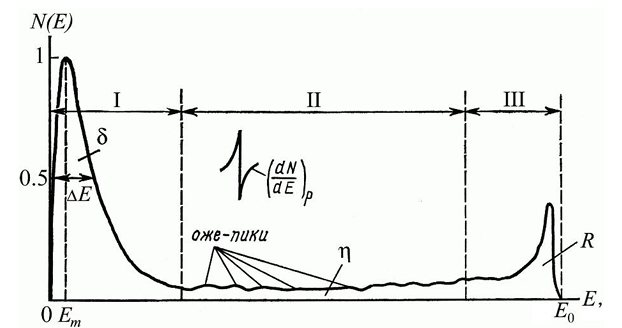
\includegraphics[width=10cm]{p1.png}
    \caption{Энергетический спектр вторичных электронов}
    \label{img_energy_levels}
\end{figure}

Небольшие пики в областях 1 и 2 обусловлены оже - электронами.

\textbf{Ожэ - электроны} - это электроны, испускаемые атомом в процессе безызлучательного перехода (автоионизации). Когда первичный электрон выбивает электрон с внутренней оболочки атома, образовавшаяся вакансия заполняется электроном с более высокого энергетического уровня. Выделившаяся при этом энергия не излучается в виде рентгеновского фотона, а передается третьему электрону (из той же или вышележащей оболочки), который преодолевает работу выхода и покидает атом. Этот вылетевший электрон и называется оже-электроном.

\subsection{Генерация рентгеновского излучения}

Механизм обарзования ожэ - электронов представлен на рисунке 2. Если процесс не пошел по пути образования ожэ - электронов, то будет происходить генерация характеристического рентгеновского излучения (рис. 3).



\newpage

\begin{figure}[h]
    \centering
    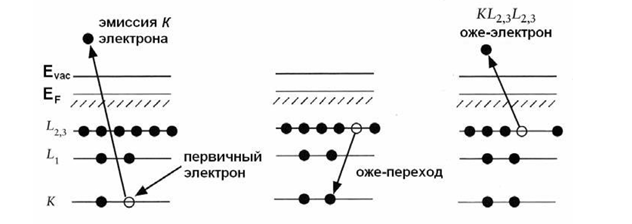
\includegraphics[width=12cm]{p3.png}
    \caption{Схема образования оже-электрона}
    \label{img_energy_levels}
\end{figure}


\begin{figure}[h]
    \centering
    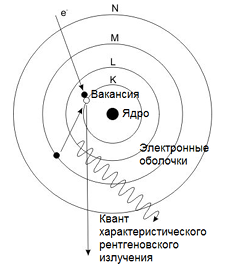
\includegraphics[width=8cm]{p2.png}
    \caption{Схема образования характеристического рентгеновского излучения}
    \label{img_energy_levels}
\end{figure}

\subsection{Линейчатый спектр, К-излучение и его эффективность}

Спектр излучения атомов довольно сложен. Наиболее простыми для определения оказались линии, соответствующие переходам между самыми глубокими уровнями. Это оболочки \textbf{K,L,M}.


Энергию электронов на таких уровнях можно оценить:

\[
E \sim R_I Z^2, \tag{4}
\]
где $R_I = 13{,}6$~эВ~--- энергия Ридберга, а $Z$~--- атомный номер.

Более точно энегрию характеристического излучения описывает \textbf{закон Мозли}:

\[
E = R_{\mathrm{I}} (Z - \sigma)^2 \left( \frac{1}{n_1^2} - \frac{1}{n_2^2} \right).\tag{5}
\]

Коэффициент $\sigma$ достаточно универсален и равен $1{,}13$ для линий K$_\alpha$ для атомов с $20 < Z < 30$.

\newpage

\subsection{Электронная ионизация ударом}

Длина волны излучения, соответствующего переходам между ближайшими к ядру оболочками, лежит в рентгеновском диапазоне. Однако для того, чтобы \textbf{вызвать переходы на нижний K-уровень}, необходимо освободить эту оболочку от электрона. В случае рентгеновского микроанализа эта ионизация делается \textbf{электронным ударом}.


Электрон пучка с энергией несколько кэВ выбивает из атома K-электрон (или переводит его на один из высоких свободных уровней), образуя вакансию. На образовавшуюся незанятую оболочку переходит один из L- или M-электронов, испуская рентгеновский фотон.

Эффективность такого способы мала по следующим причинам:

\begin{itemize}
  \item  электроны зонда в основном взаимодействуют не с глубокой К-оболочкой, а с внешними электронами атома
  \item  не всякая вакансия на К-оболочке приводит к эмиссии рентгеновского излучения.
  \item  при взаимодействии электрона с зарядом ядра происходит торможение электрона, а его потерянная энергия высвечивается в виде непрерывного (белого) фона рентгеновского излучения, называемого \textbf{тормозным}. 
\end{itemize}

Непрервный рентгеновский спектр описывается формулой:

\[
N(E) = \frac{a Z (E_0 - E)}{E}.\tag{6}
\]

Эта формула определяет число электронов в 1 с на единичный интервал  энергий и на один падающий электрон с энергией $E_0$

\subsection{Количественный микроанализ и искажающие его факторы}

Необходимо знать эффективность 
рентгеновского излучения отдельных атомов под действием электронного 
удара.

Это можно сделать через сравнение интенсивности излучения эталонного элемента $I_0$ с имеющейся I. Далее находят концентарция данных атомов в образце $C$

\[
\frac{C}{C_0} = \frac{I}{I_0}.\tag{7}
\]

Более лучшая формула, которая дает большее согласие с опытом (\textbf{Второе приближение кастена})

\[
\frac{I_{\text{обр}}}{I_{\text{эт}}} = \frac{c_A \alpha_A}{\sum_i c_i \alpha_i},\tag{8}
\]

Она тем не менее не учитывает эффектов поглощения излучения и флуоресценции.


Следующим важным шагом в количественном рентгеновском поле приближения Кастена является применение метода ZAF-коррекции.

ZAF расшифровывается как:

\begin{enumerate}
    \item Атомного номера $Z$.
    \item Поглощения излучения в образце (\textit{Absorption}).
    \item Флуоресценции (\textit{Fluorescence}).
\end{enumerate}

\newpage

\subsection{Электронный зонд}

Источником электронов в приборе JOEL JSM-7001F служит \textbf{вольфрамовый термополевой катод}.


 
С увеличением температуры нити возрастает эмиссия электронов, которая, однако, достигает насыщения при некоторой температуре и остается постоянной при дальнейшем нагреве. С помощью напряжения смещения между катодом и \textbf{цилиндром Венельта} можно регулировать уровень 
тока насыщения. 


Далее, по ходу пучка, на расстоянии около 10 мм от цилиндра Венельта, располагается анодная пластина

Анод 
заземляется, а на катод подаётся отрицательное напряжение от 1 до 30 кВ.

На участке от цилиндра Венельта до анода происходит ускорение электронов.


Катод, цилиндр Венельта и анод образуют \textbf{трёхэлектродную пушку}, 
траектории электронов в которой схематически показаны на рис


\begin{figure}[h]
    \centering
    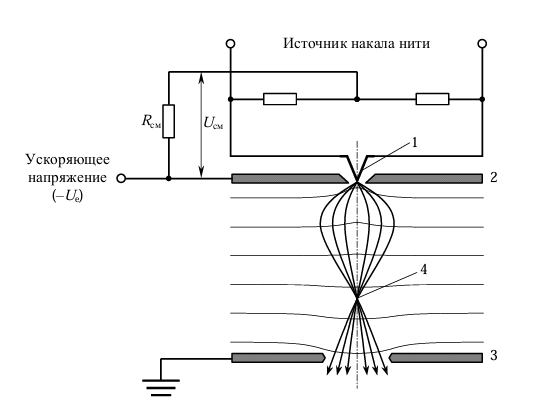
\includegraphics[width=12cm]{p6.png}
    \caption{Схематическое изображение электронной пушки и траектории электронов в ней: 1 — катод, 2 — венельт, 3 — анод, 4 — кроссовер }
    \label{img_energy_levels}
\end{figure}

Пройдя через отверстие в анодной платине, электроны попадают в систему электромагнитных линз, при помощи которых формируется \textbf{узкий зонд}. Линзы представляют собой соленоиды, соосные электронному пучку. Схематически линза изображена на рис.
Она представляет собой 
цилиндрически симметричный электромагнит с очень острыми кольцевыми наконечниками полюсов, который создает в малой области очень 
сильное неоднородное магнитное поле, которое фокусирует электроны, 
летящие вертикально через эту область.


При создании узкого зонда необходимо, чтобы в целом электронная 
оптика давала бы на образце уменьшенное изображение источника электронов — кроссовера электронной пушки.

используются квадрупольные линзы (рис. 5 б) и октупольные линзы. Эти линзы используются 
не как усиливающие, а как корректирующие, например, астигматизм.


На рисунке 6 изображено, как расходящиеся электроны собираются в параллельный пучок. 
Действие такого устройства подобно работе оптической линзы, когда объект находится не в фокусе.
\newpage

\begin{figure}[h]
    \centering
    \begin{minipage}{0.45\textwidth}
        \centering
        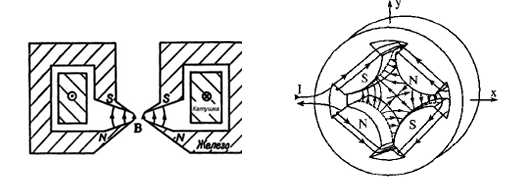
\includegraphics[width=\linewidth]{p7.png}
        \caption {Магнитные линзы: а)  двухполюсная б) квадрупольная}
        \label{fig:image1}
    \end{minipage}
    \hfill
    \begin{minipage}{0.45\textwidth}
        \centering
        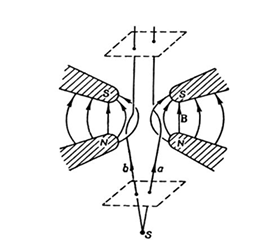
\includegraphics[width=\linewidth]{p8.png}
        \caption{Движение электрона в магнитной линзе}
        \label{fig:image2}
    \end{minipage}
\end{figure}

\subsection{Детектор рентгеновского излучения}

Электронный зонд, достигая поверхности образца, вызывает рентге
новское излучение. Для проведения микроанализа необходимо получить 
спектральную зависимость этого излучения.


Есть два типа детекторов:

\begin{itemize}
  \item волновой - с более высоким разрешением
  \item энерго - дисперсионный - более быстродействующий
\end{itemize}

\textbf{Волновой детектор}


Основным элементом волнового детектора является  монохроматор, 
который  выделяет из полного потока излучения, излучение лишь определенной длины волны. Роль такого монохроматора играют специальные 
кристаллы-анализаторы.


Здесь применяется закон Брегга - Вульфа:

\[
\lambda n = 2d \sin \theta,\tag{9}
\]

Значит, можно разместить детктор так, как нужно, чтобы в него попадали кванты определенной энергии. Обычно такое положение находится в \textbf{круге Роуланда}


Для регистрации рентгеновского излучения в диапазоне от 0,18~кэВ до 0,5~кэВ (от 90~\AA{} до 20~\AA), используя кристалл-анализатор STE, необходимо около 20~минут. Поэтому волновой детектор используют в основном для уточнения отдельных участков спектра, получаемого с помощью \textbf{энергодисперсионного детектора}.


\textbf{Энергодисперсионный детектор}

Энергодисперсионный детектор преобразует энергию каждого фотона 
рентгеновского излучения в пропорциональный энергии сигнал напряжения.Этот процесс происходит в три стадии:

\newpage

\begin{itemize}
  \item рентген производит ионизацию атомов $\Rightarrow $ обрвзуются электороны и дырки
  \item с помощью предусилителя на полевом транзисторе неравномерный заряд преобразуется в сигнал напряжения
  \item сигнал для измерения поступает на вход импульсного процессора
\end{itemize}

\section{Экспериментальная установка
}

Микроскоп, изучаемый в ходе данной работы, позволяет вести 
наблюдения образца в трех основных режимах: во вторичных электронах, 
в отраженных электронах, в рентгеновских лучах (микроанализатор).

\begin{figure}[h]
    \centering
    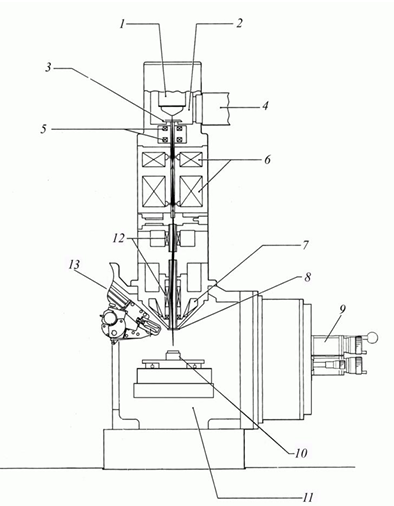
\includegraphics[width=8cm]{p4.png}
    \caption{ Общая схема растрового электронного микроскопа: 
1 — электронная пушка; 2 — камера электронной пушки; 
3 — анод; 4 — вакуумная магистраль; 5 — юстировочные катушки; 6 —
конденсорные линзы; 7 — объектная линза; 8 — детектор упругоотражённых 
электронов; 9 — система позиционирования образцов; 10  — держатель образцов; 
11 — основная вакуумная камера; 12 —  сканирующие катушки; 13 —
рентгеновский спектрометр }
    \label{img_energy_levels}
\end{figure}

\subsection{формирование изображения в РЭМ}

Изображение получается не целиком, а формируется поточечно. Об
лучая тонким электронным пучком одну точку на образце, мы в одном 
режиме регистрируем истинно вторичные электроны, а в другом — упругоотражённые, которые содержат информацию об этой точке.


 Для того чтобы получить 
целостную картину, необходимо сканировать поверхность образца электронным зондом, проводя измерения последовательно в каждой точке.  
В итоге получается растровое изображение, которое и выводится на 
экран.


Размер исследуемой растровым микроскопом «точки» не может быть меньше 100~\AA.


Частота сканирования и число строк могут изменяться в широких 
пределах. При этом качество изображения характеризуется параметром 
«сигнал/шум», показывающим соотношение интенсивности информационного сигнала в данной точке к шумовому сигналу.



\begin{figure}[h]
    \centering
    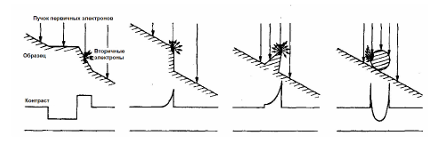
\includegraphics[width=12cm]{p5.png}
    \caption{Зависимость формы видеосигнала РЭМ от формы изучаемого 
объекта }
    \label{img_energy_levels}
\end{figure}

\section{Ход работы}

\subsection{Получение изображения образца медь - хром}

\begin{figure}[h]
    \centering
    \begin{minipage}{0.45\textwidth}
        \centering
        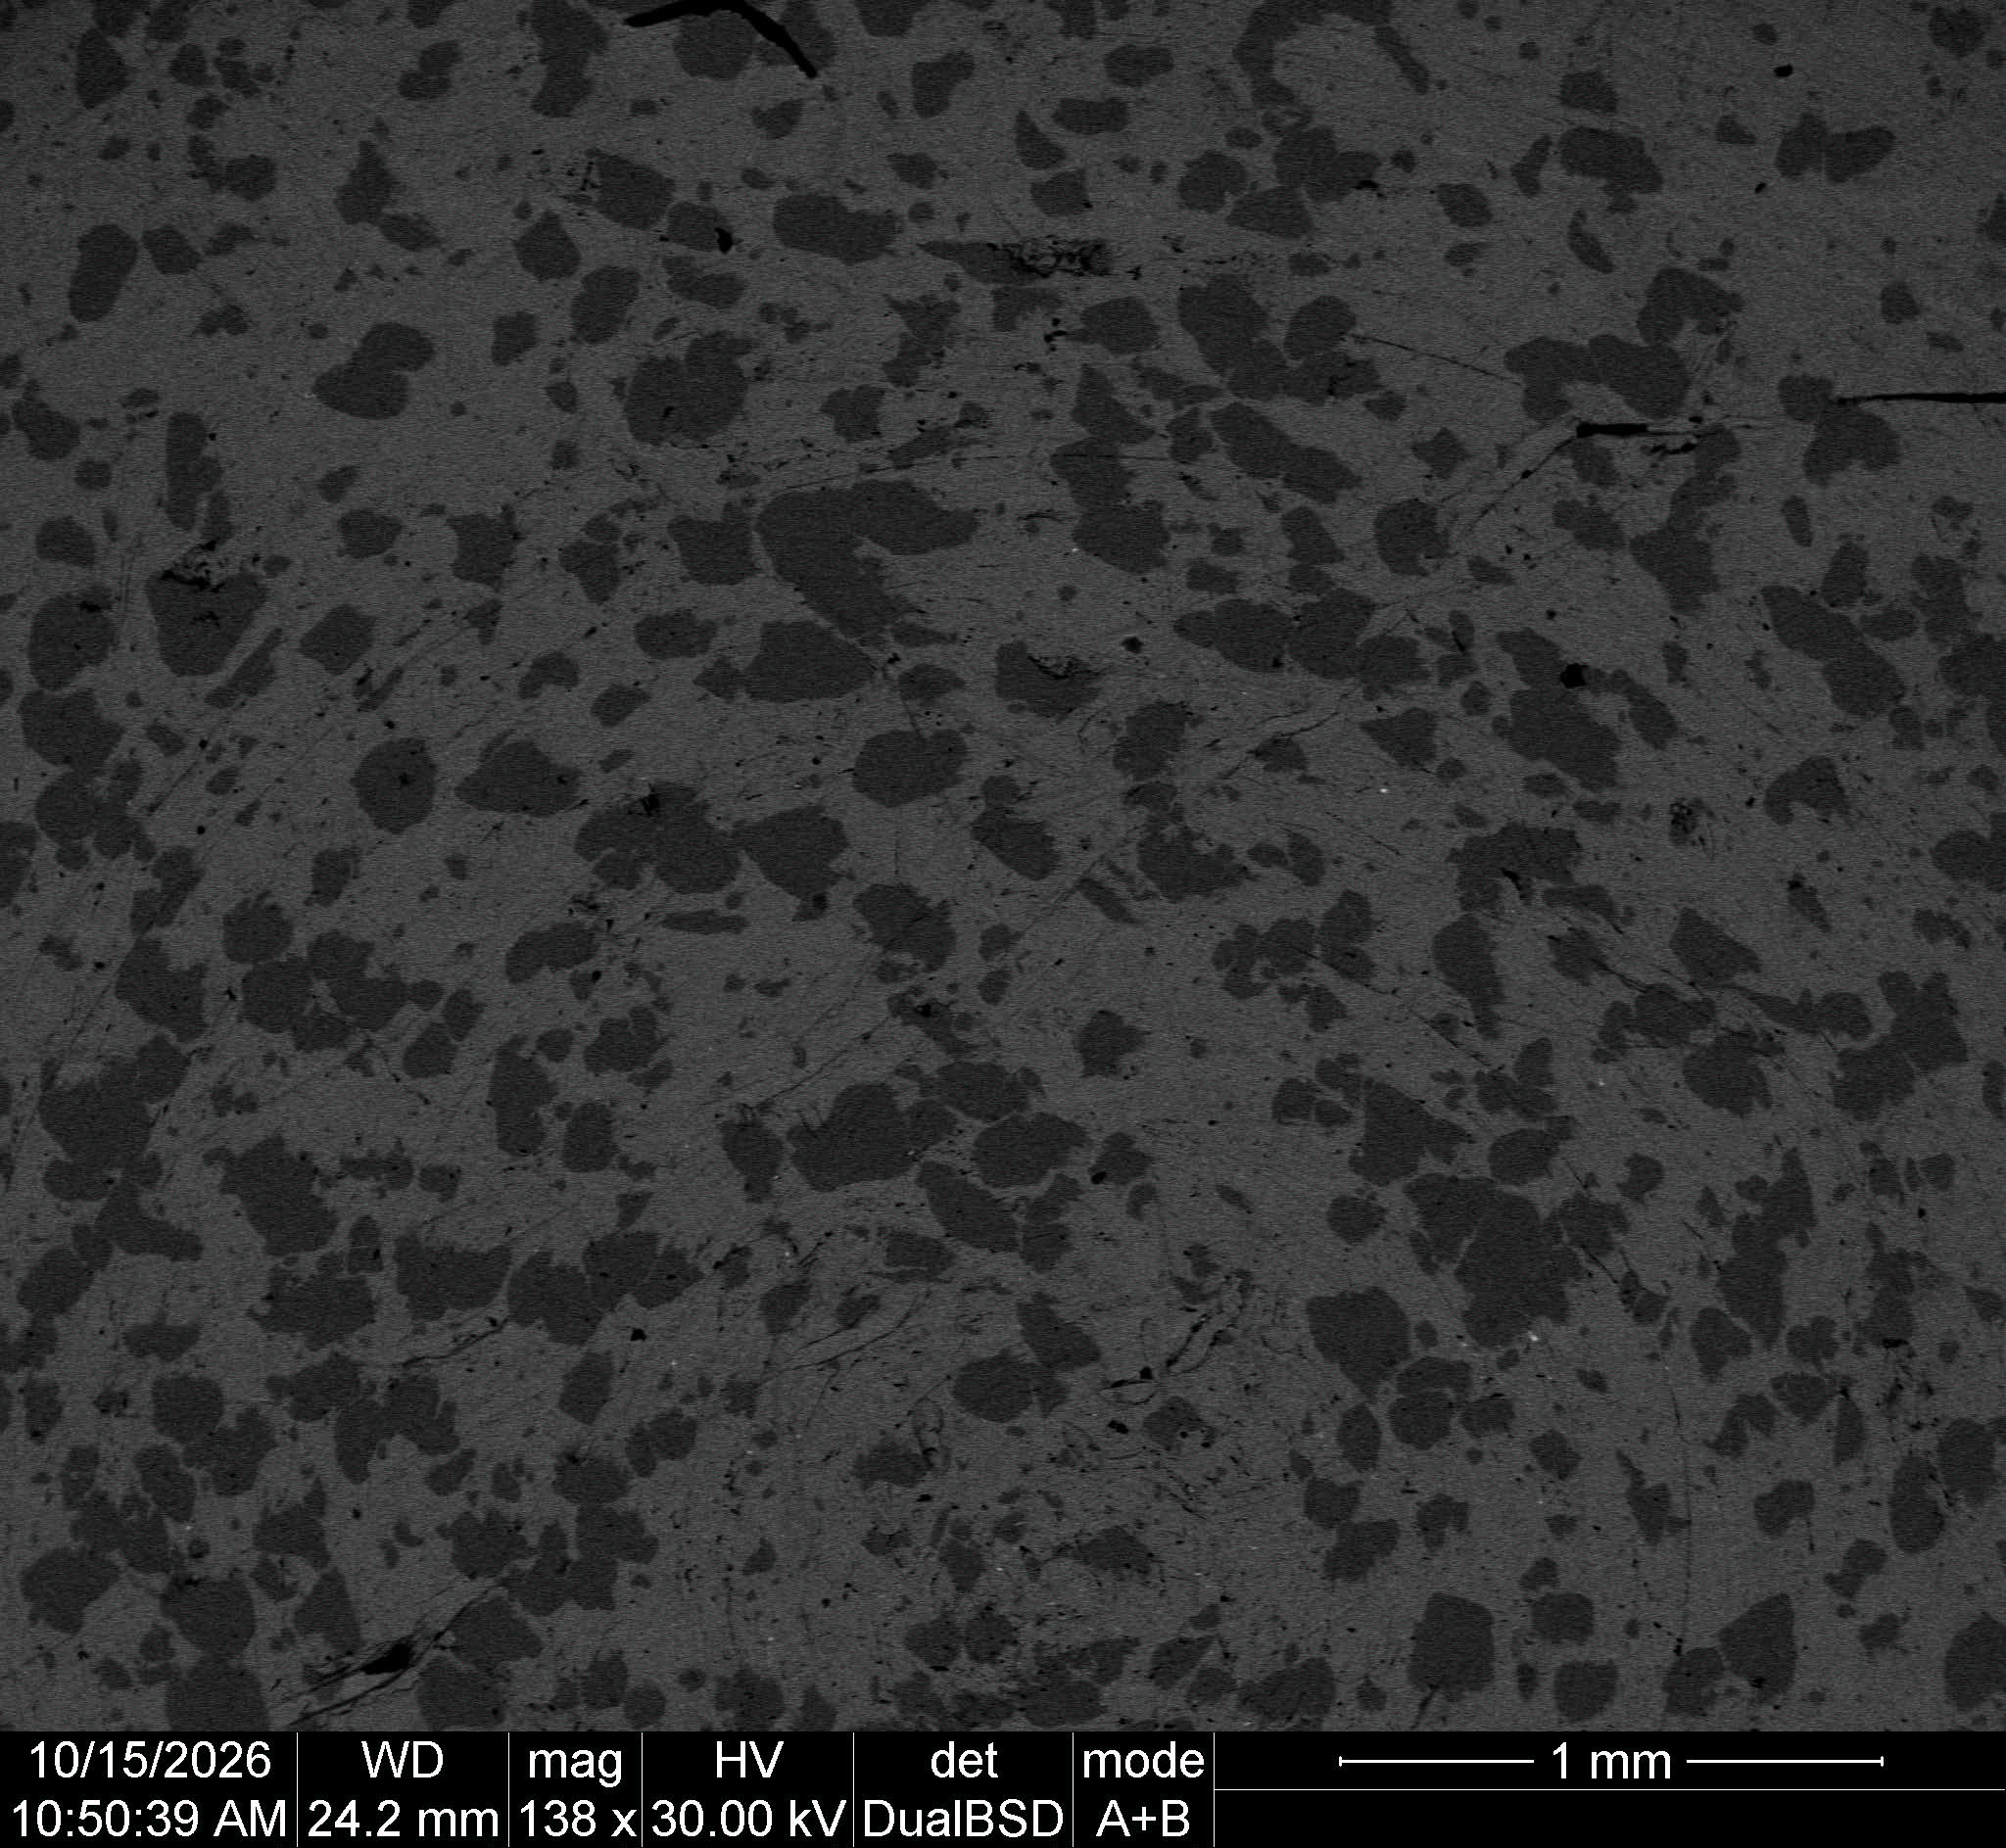
\includegraphics[width=\linewidth]{p002.jpg}
        \caption {Режим BSE - элементный контраст mode A+B}
        \label{fig:image1}
    \end{minipage}
    \hfill
    \begin{minipage}{0.45\textwidth}
        \centering
        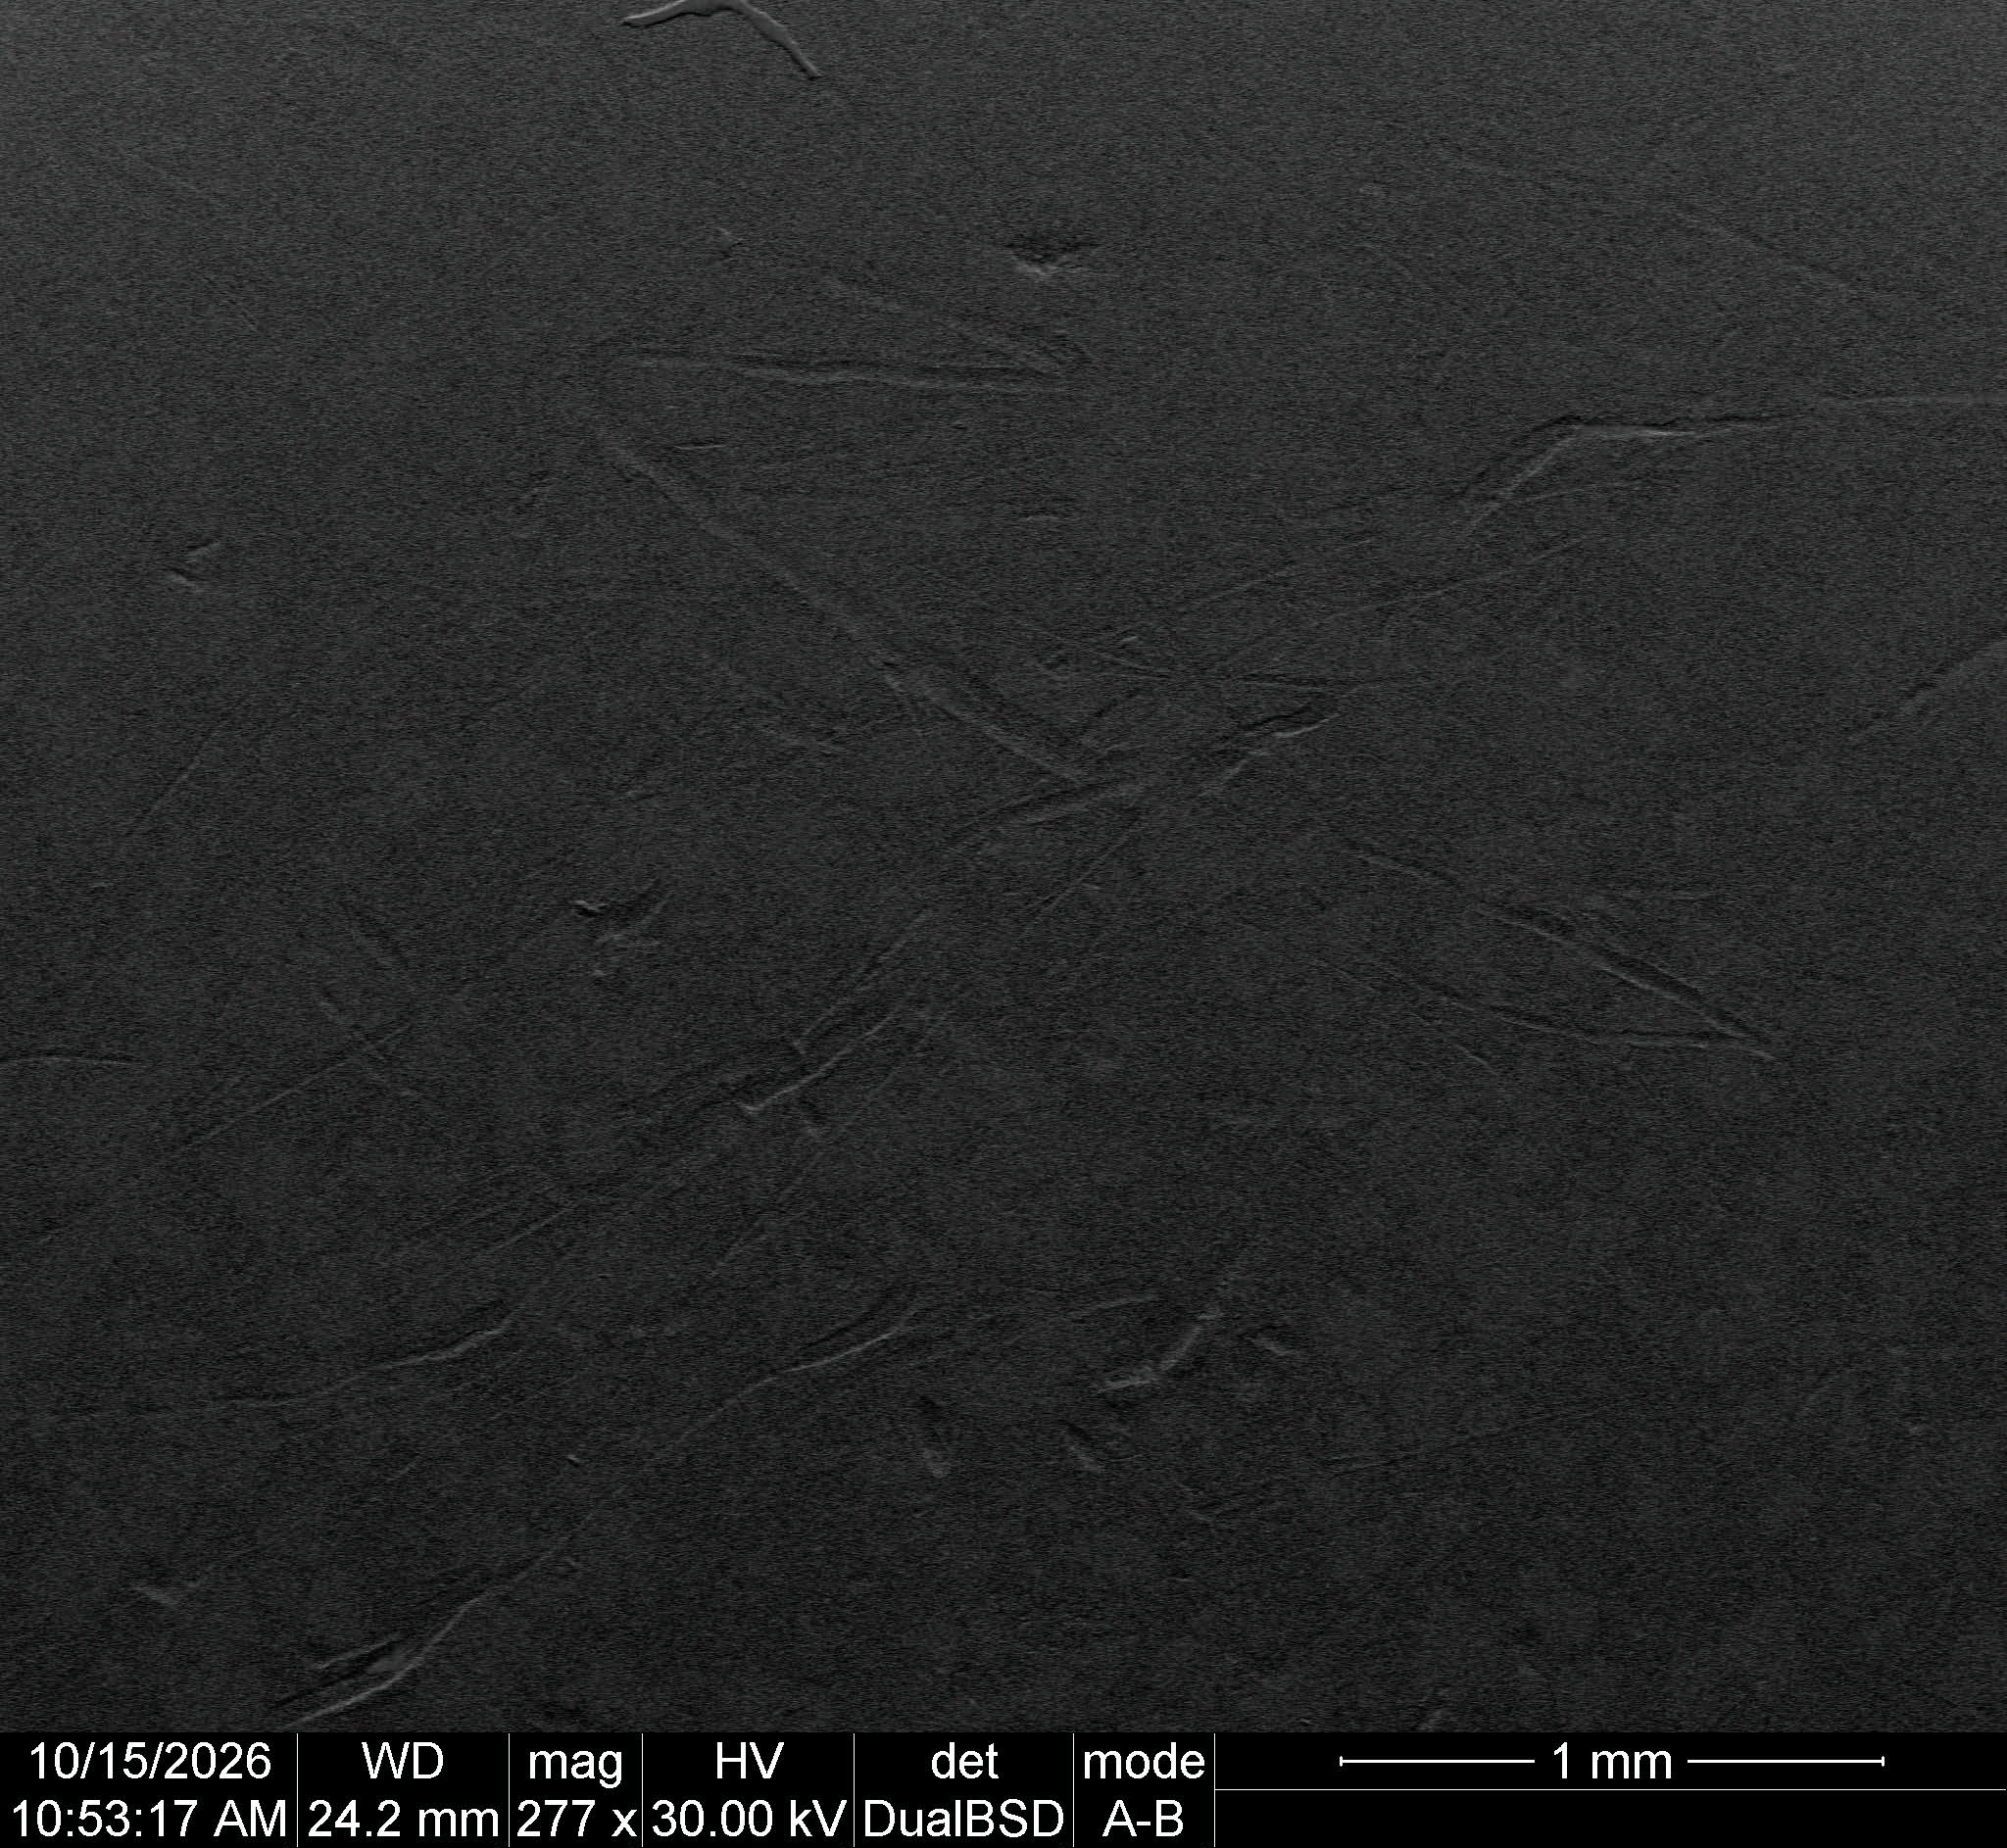
\includegraphics[width=\linewidth]{p003.jpg}
        \caption{Режим BSE - топографический контраст mode A-B}
        \label{fig:image2}
    \end{minipage}
\end{figure}
\newpage
\begin{figure}[h]
    \centering
    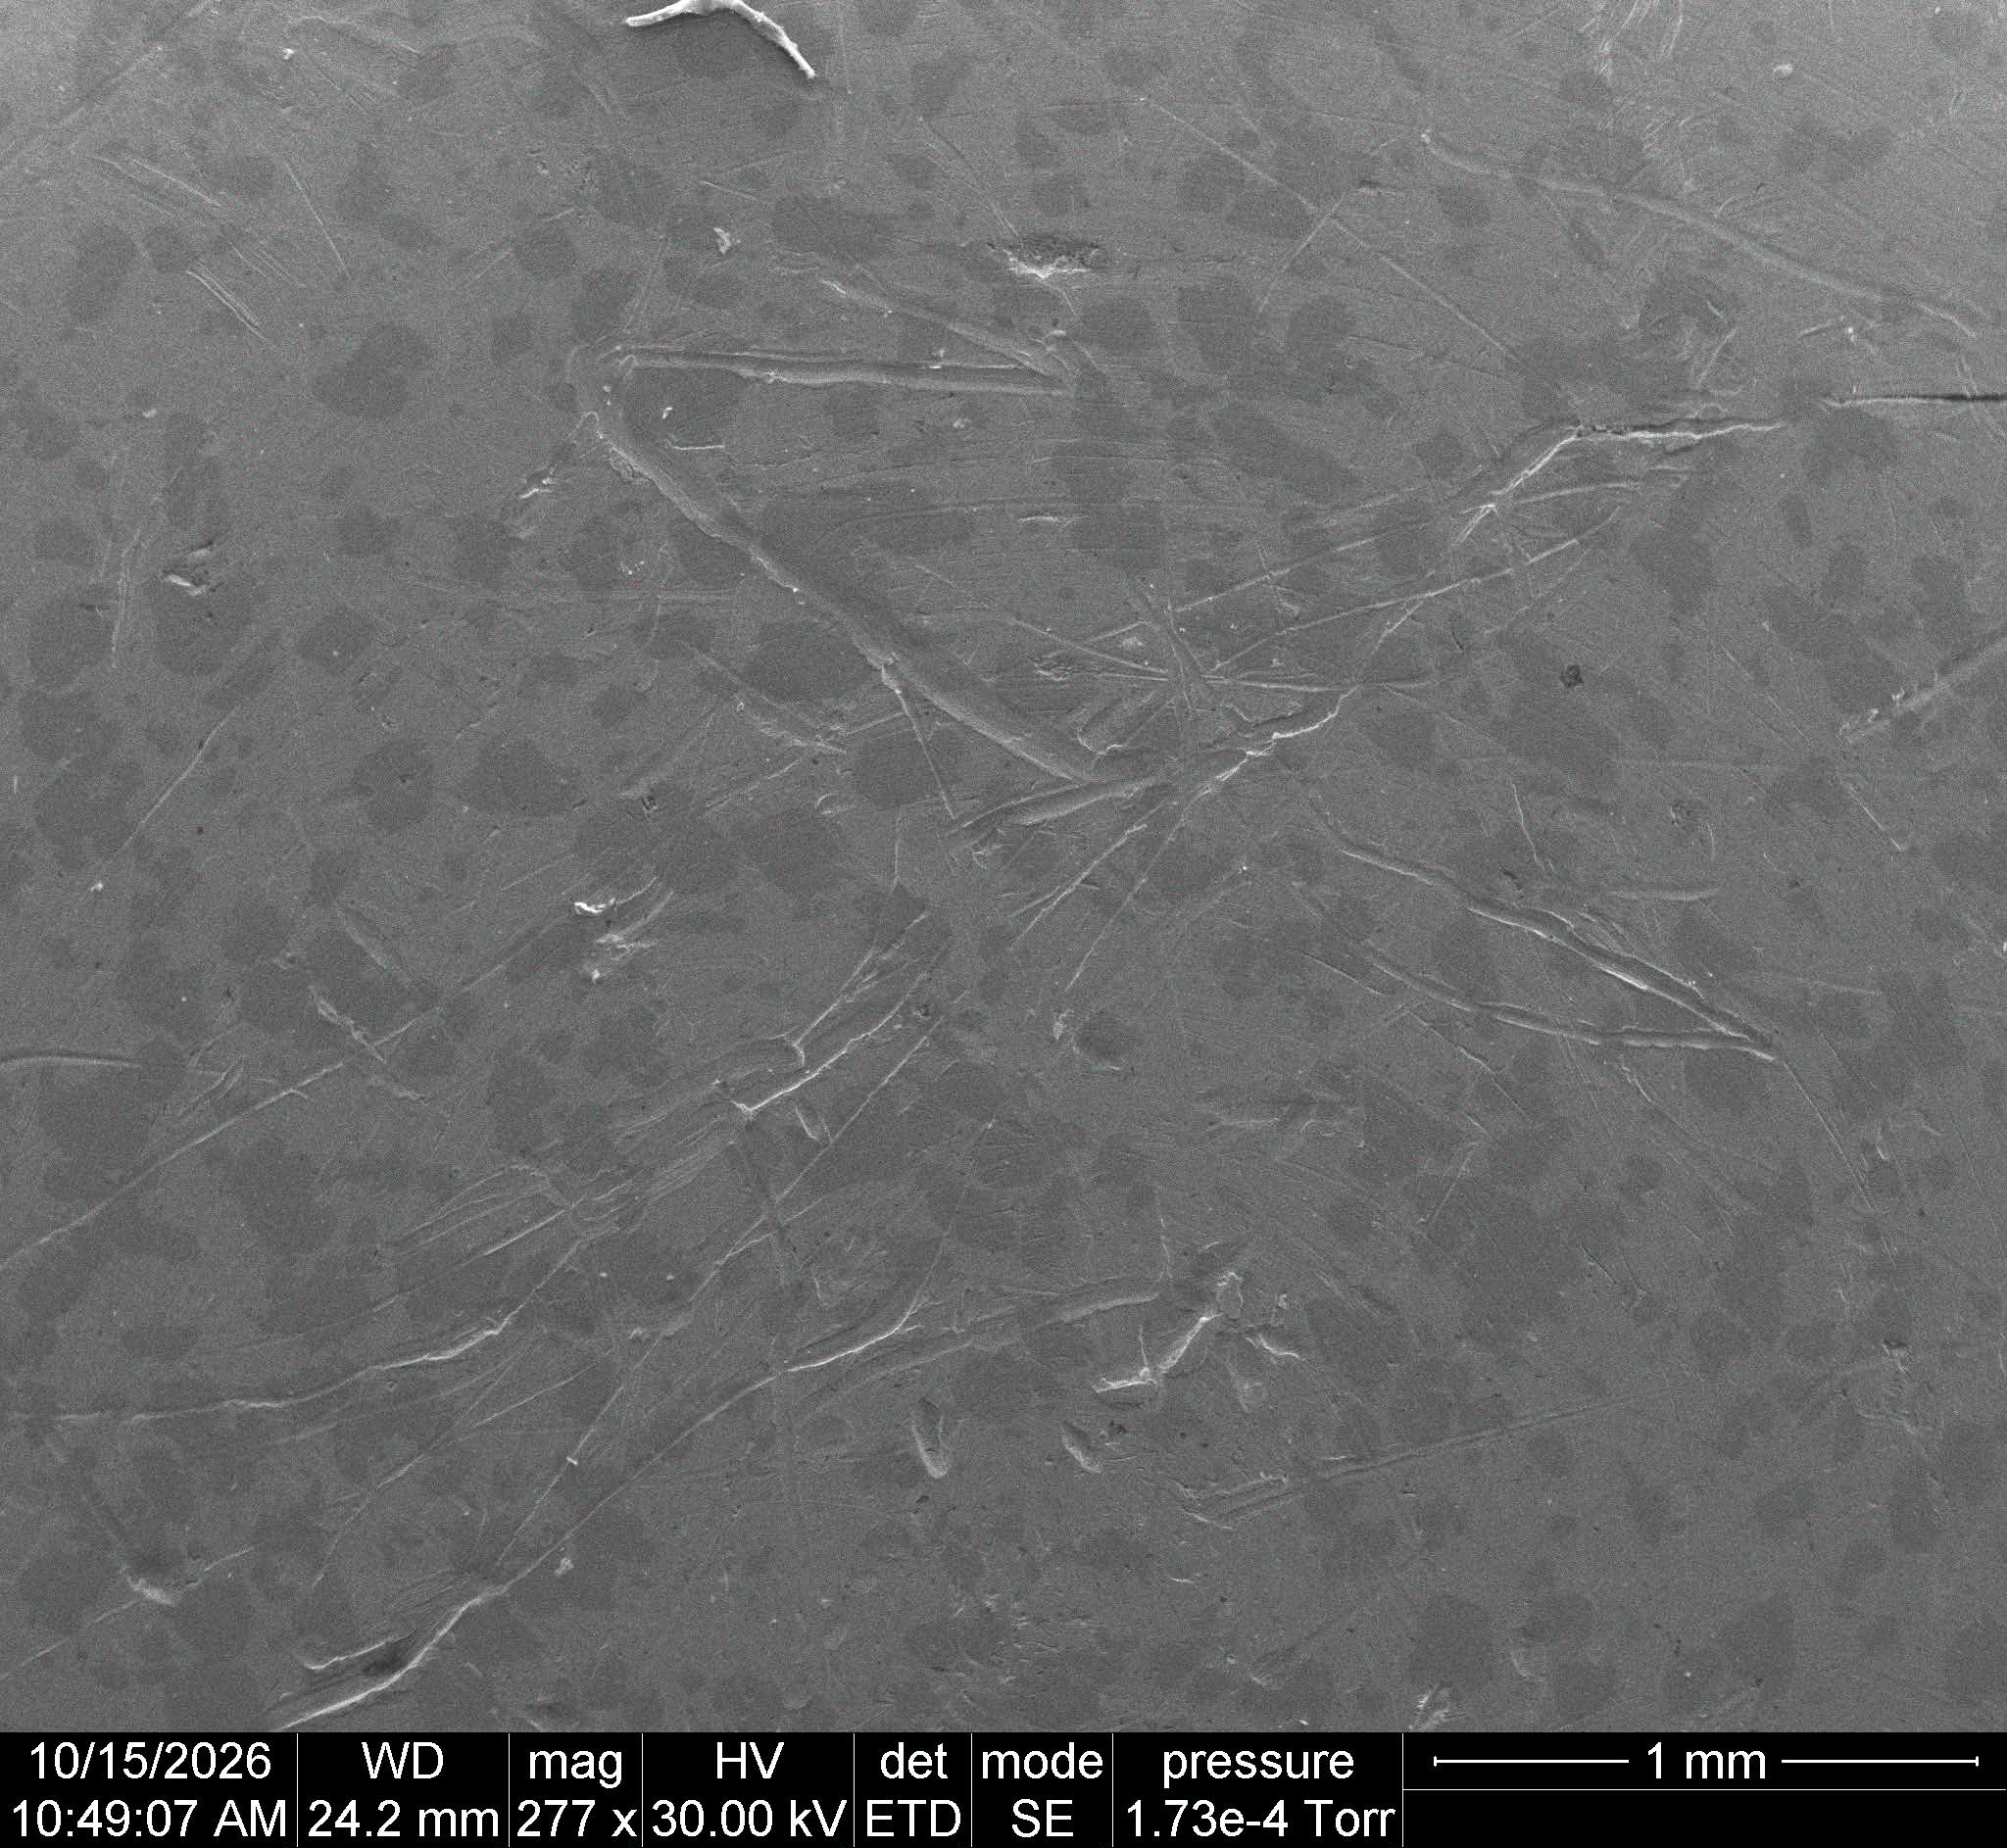
\includegraphics[width=10cm]{p001.jpg}
    \caption{Режим SE - истинно вторичные электроны}
    \label{img_energy_levels}
\end{figure}

Получили изображения образца Cu-Cr в различный режимах работы микроскопа:

\begin{itemize}
  \item \textbf{Режим A+B (элементный контраст)}:Изображение четко разделяет фазы сплава по атомному номеру (Z-контраст). Темные пятна соответствуют хрому (Z=24), а светлый фон — меди (Z=29), так как коэффициент обратного рассеяния электронов растет с увеличением атомного номера.
  \item \textbf{Режим A-B (топографический контраст)}: Сигнал, зависящий от состава, взаимно уничтожается. Изображение становится темным и однородным по цвету фаз, но на нем четко проявляются царапины и неровности поверхности (следы механической обработки/полировки).
  \item \textbf{Режим SE (вторичные электроны)}: Дает смешанную картину. Доминирует топографический контраст (хорошо видны царапины и рельеф), однако из-за выхода вторичных электронов из приповерхностного слоя также слабо различимы границы фаз (пятна), соответствующие разным элементам сплава.
\end{itemize}

\subsection{Рассмотрение диэлектрических объектов}

\begin{itemize}
  \item \textbf{Эффект зарядки диэлектриков (режим SE):} Оба изображения пенопластового шарика получены в режиме вторичных электронов (SE). Искажение и «сжатие» изображения на втором снимке шарика обусловлено накоплением отрицательного заряда на поверхности диэлектрика (пенопласта), который не имеет пути для стекания электронов. Возникающее электростатическое поле отклоняет первичный пучок и препятствует сбору вторичных электронов детектором , что приводит к 
  
  геометрическим искажениям картинки.
\end{itemize}


\newpage

\begin{figure}[h]
    \centering
    \begin{minipage}{0.45\textwidth}
        \centering
        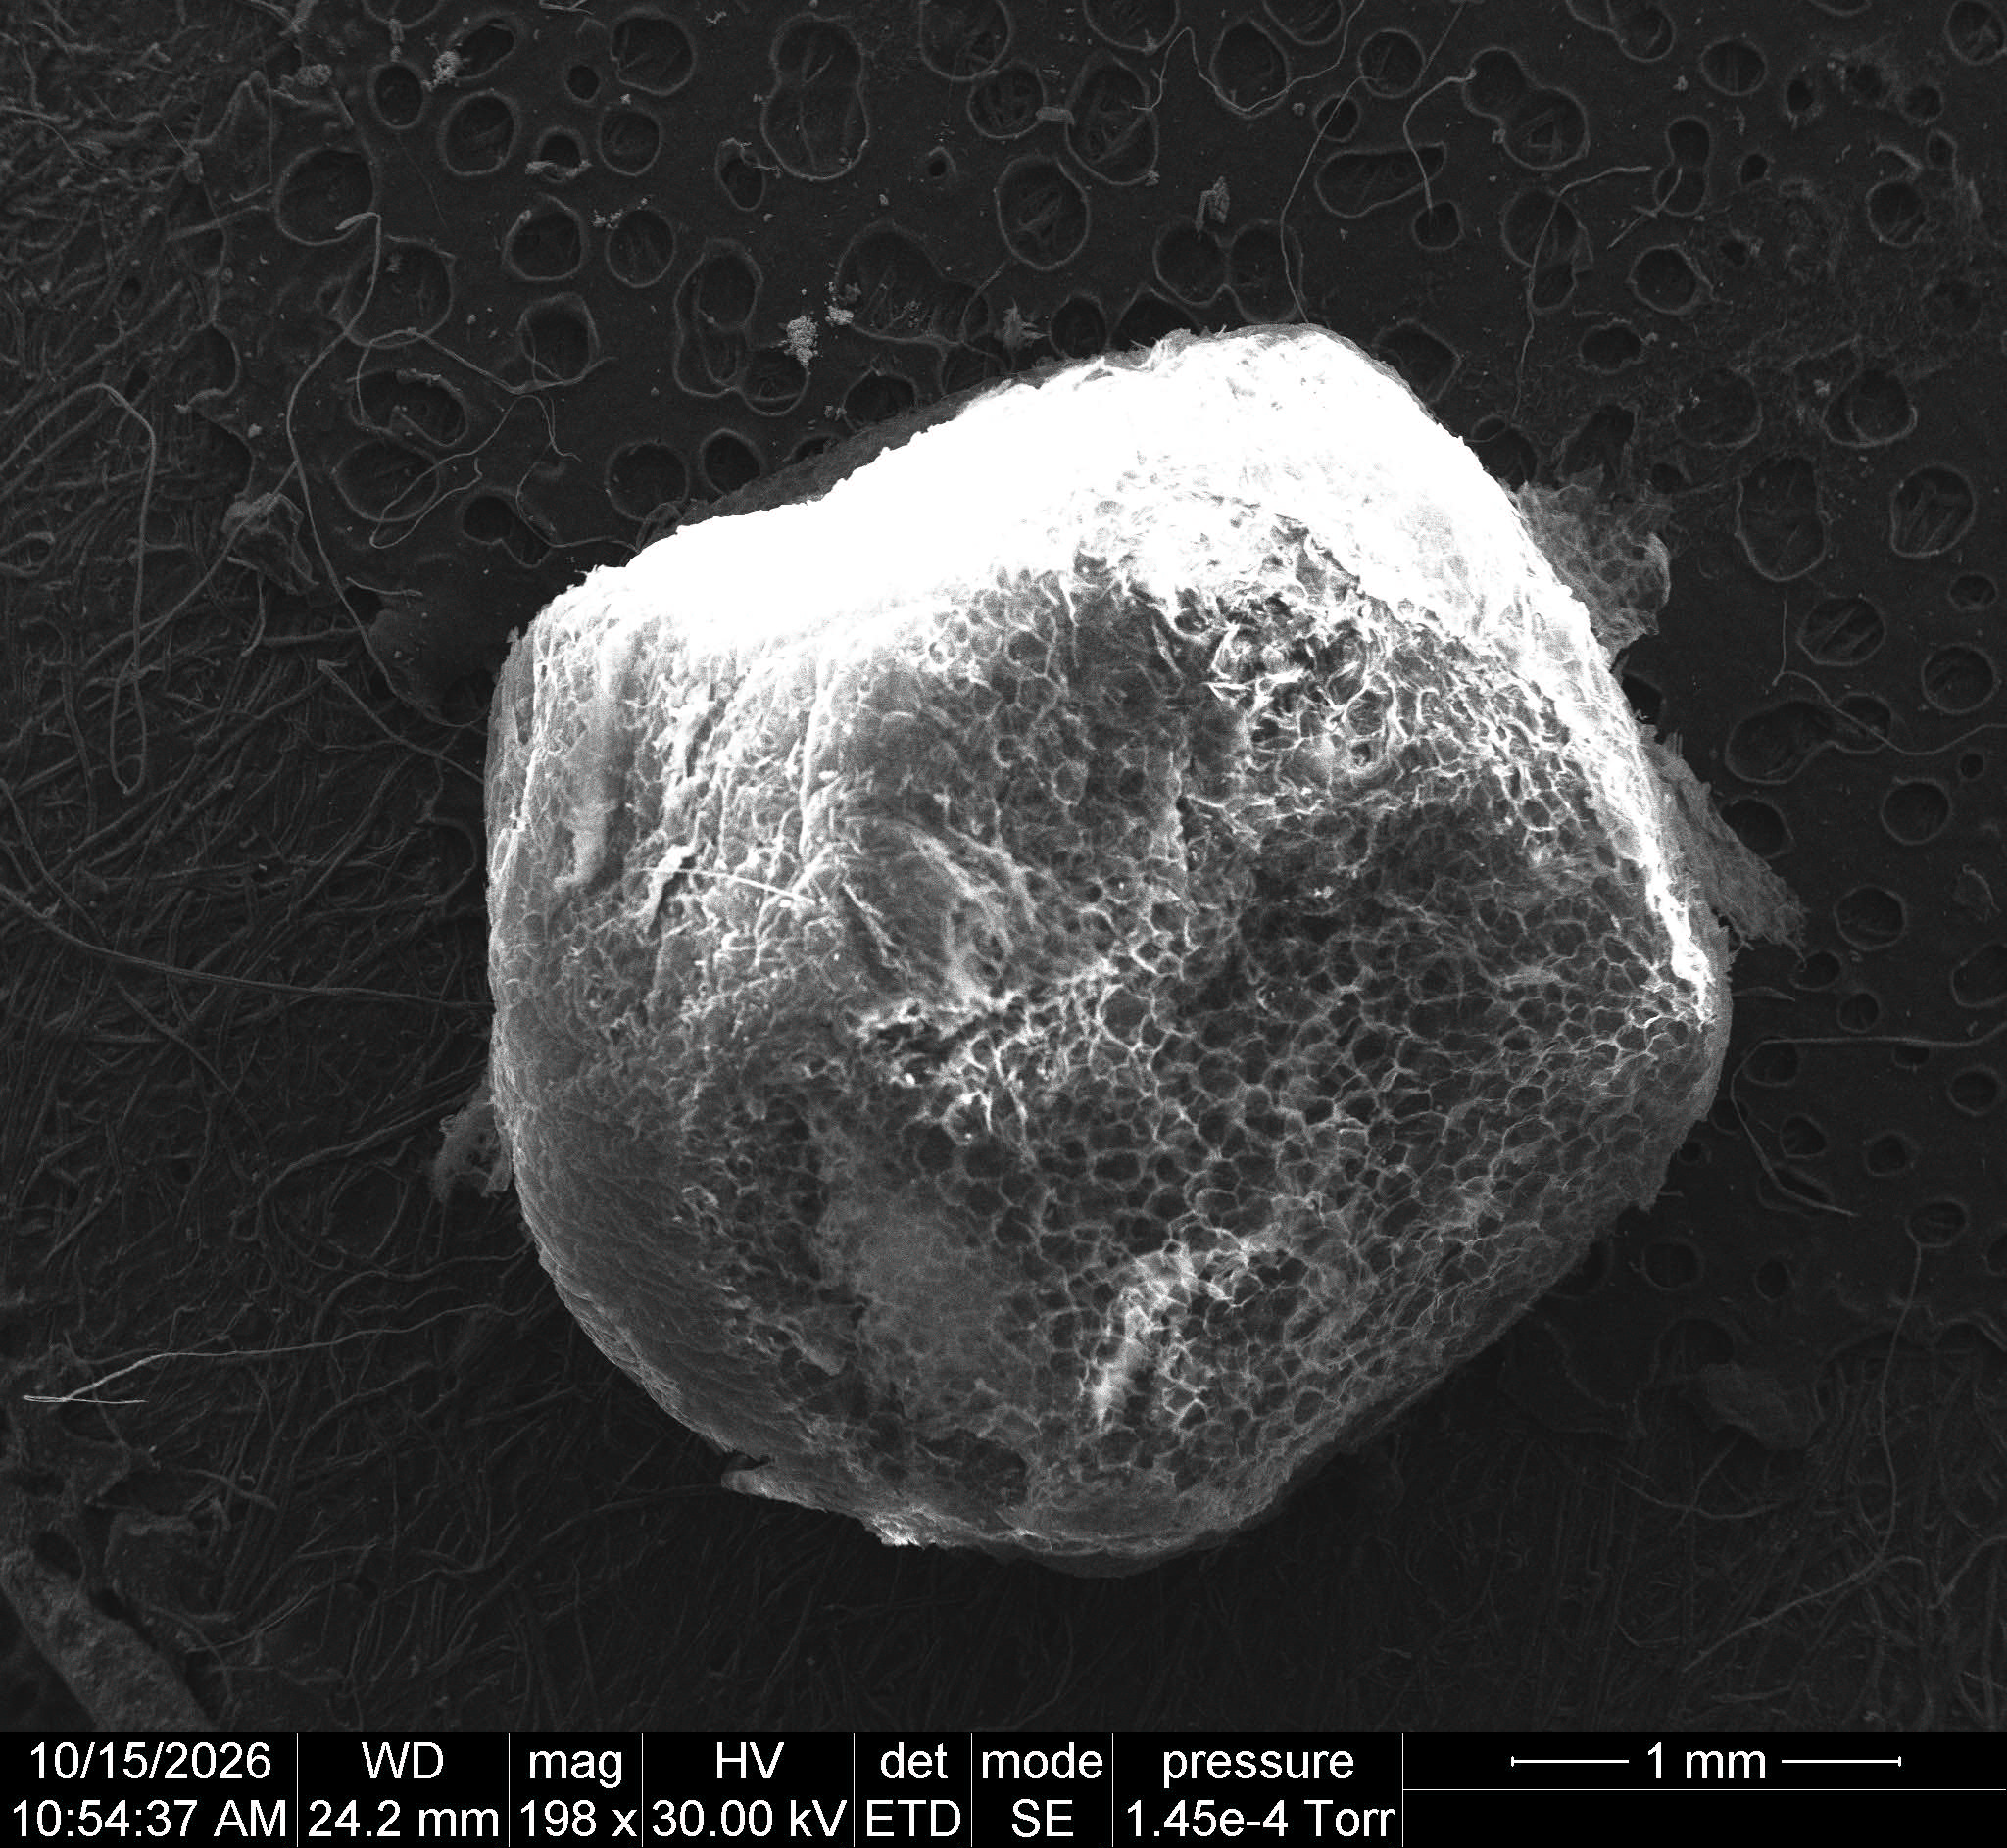
\includegraphics[width=\linewidth]{pp1.jpg}
        \caption {Пенопластовый шарик}
        \label{fig:image1}
    \end{minipage}
    \hfill
    \begin{minipage}{0.45\textwidth}
        \centering
        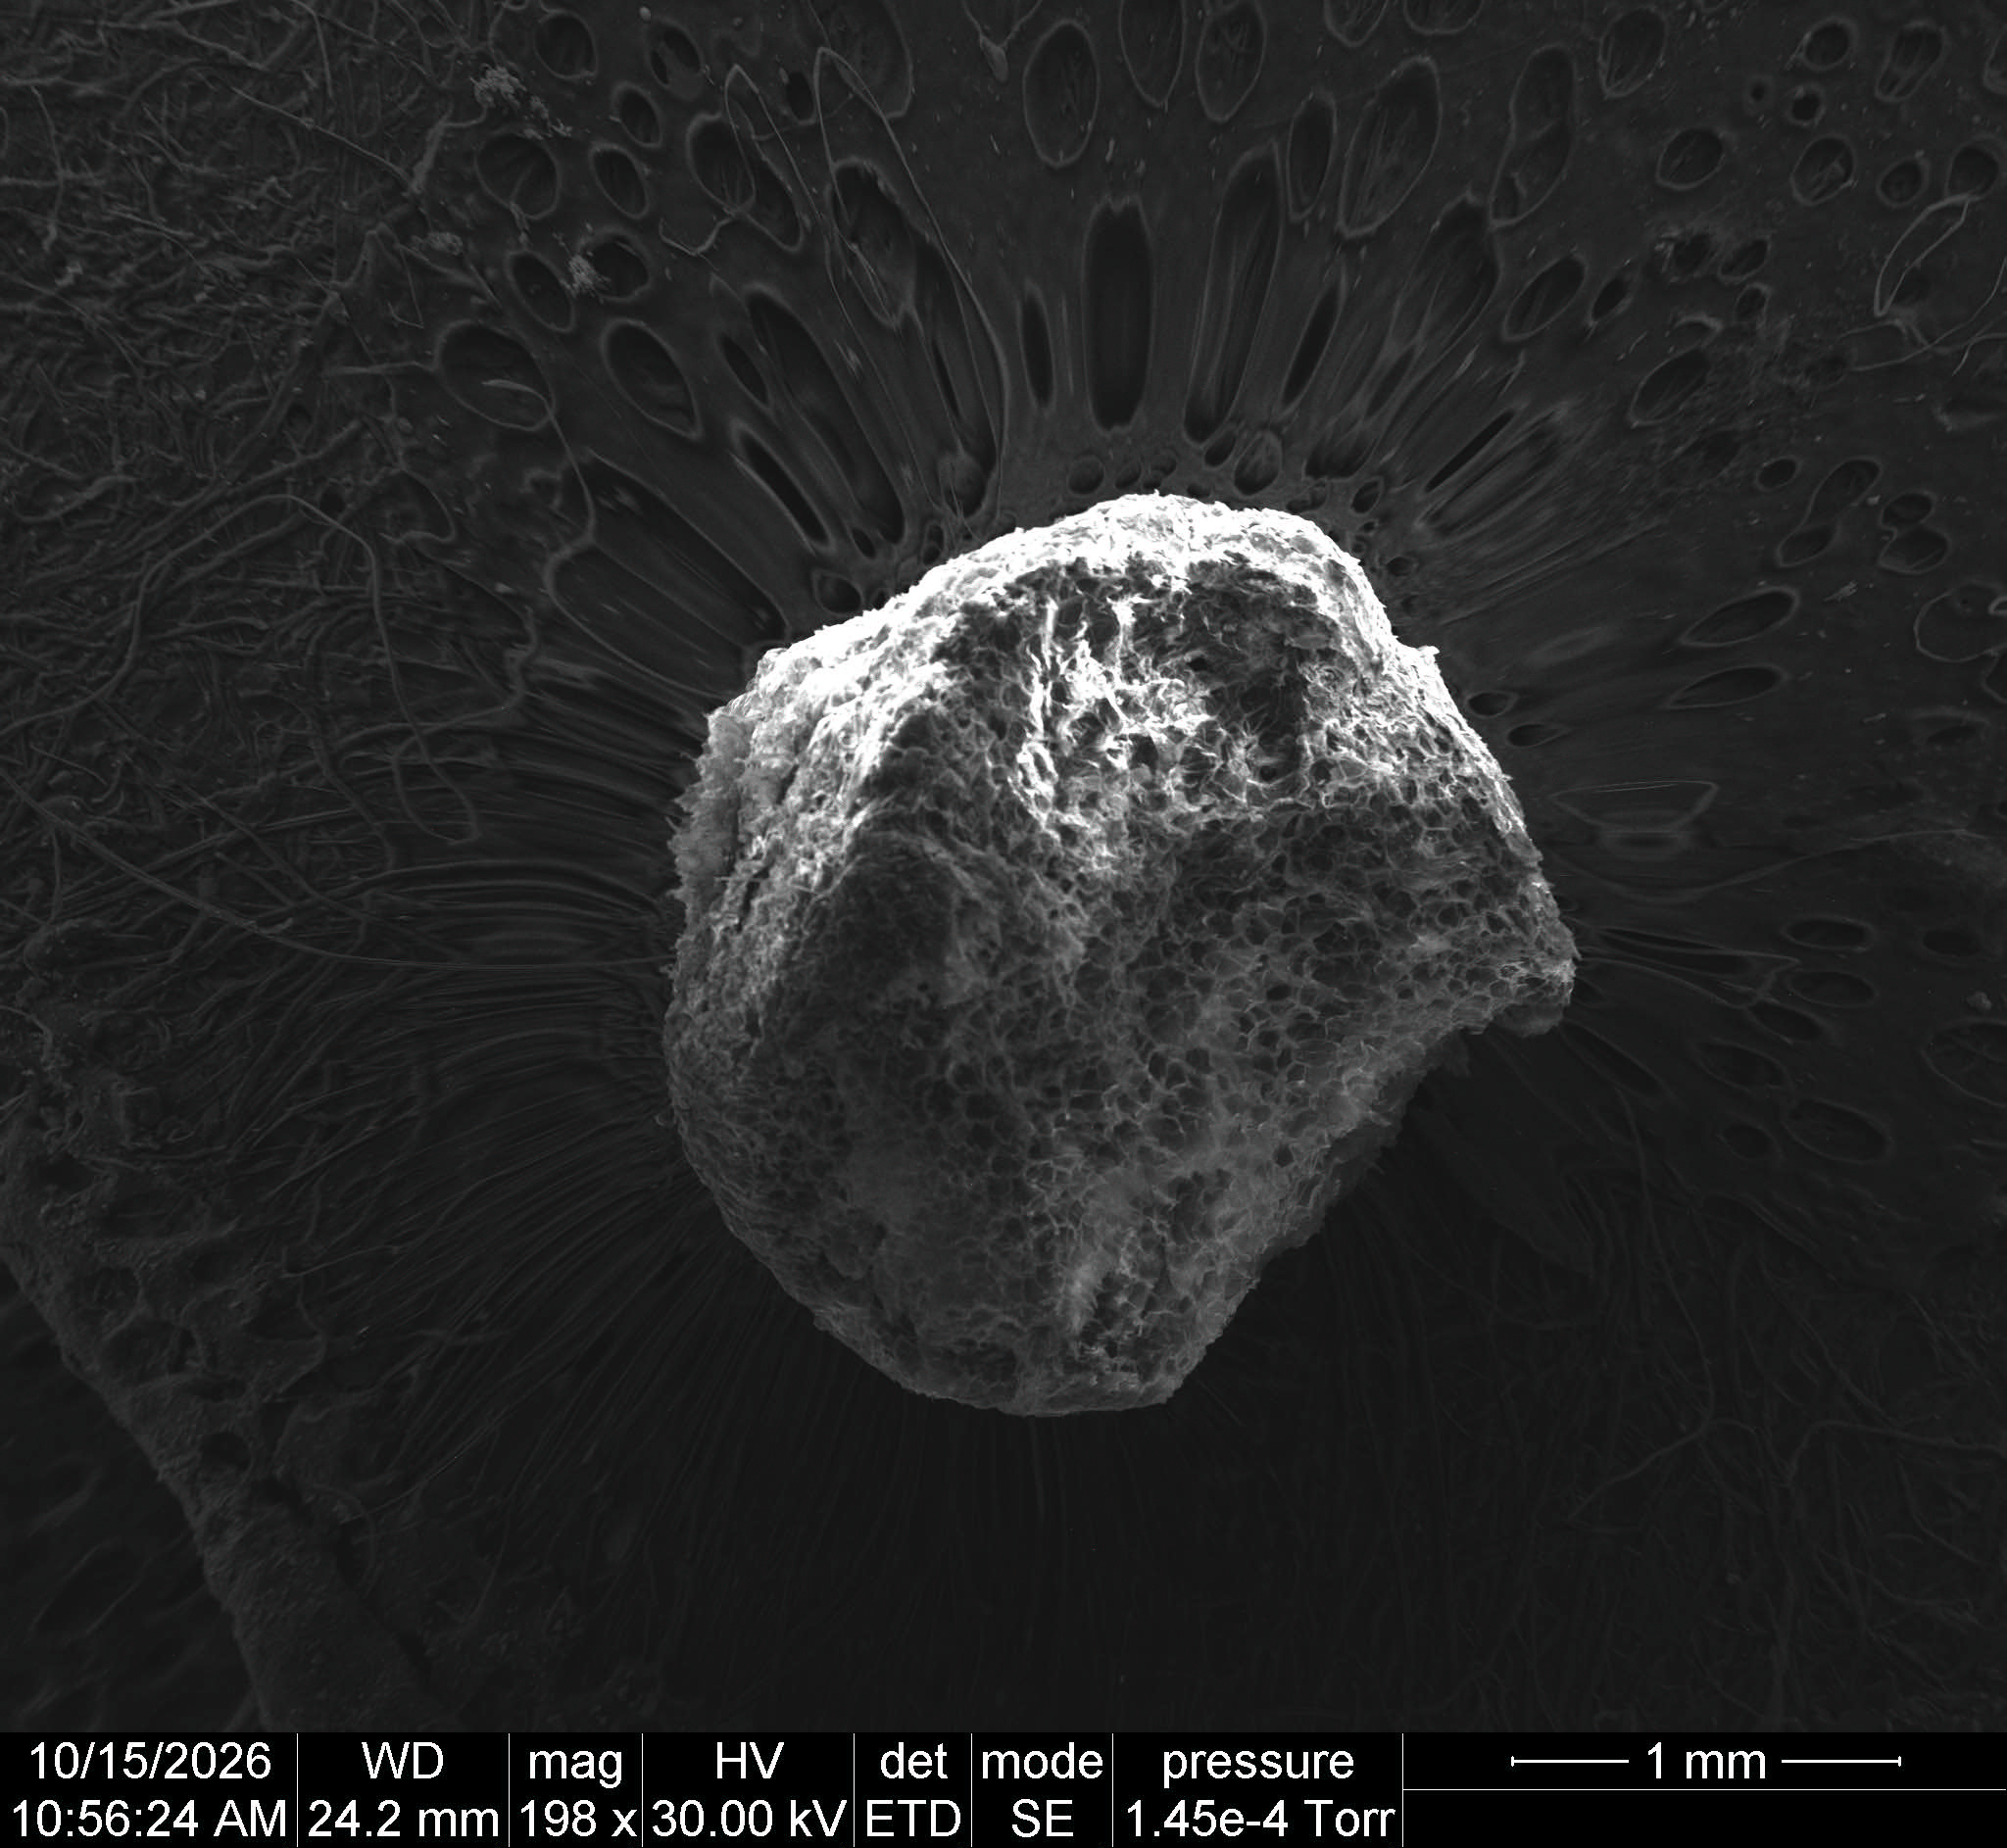
\includegraphics[width=\linewidth]{pp2.jpg}
        \caption{Заряженный пенопластовый шарик}
        \label{fig:image2}
    \end{minipage}
\end{figure}

\subsection{Разные картинки разных вещей}

\begin{figure}[h]
    \centering
    \begin{minipage}{0.45\textwidth}
        \centering
        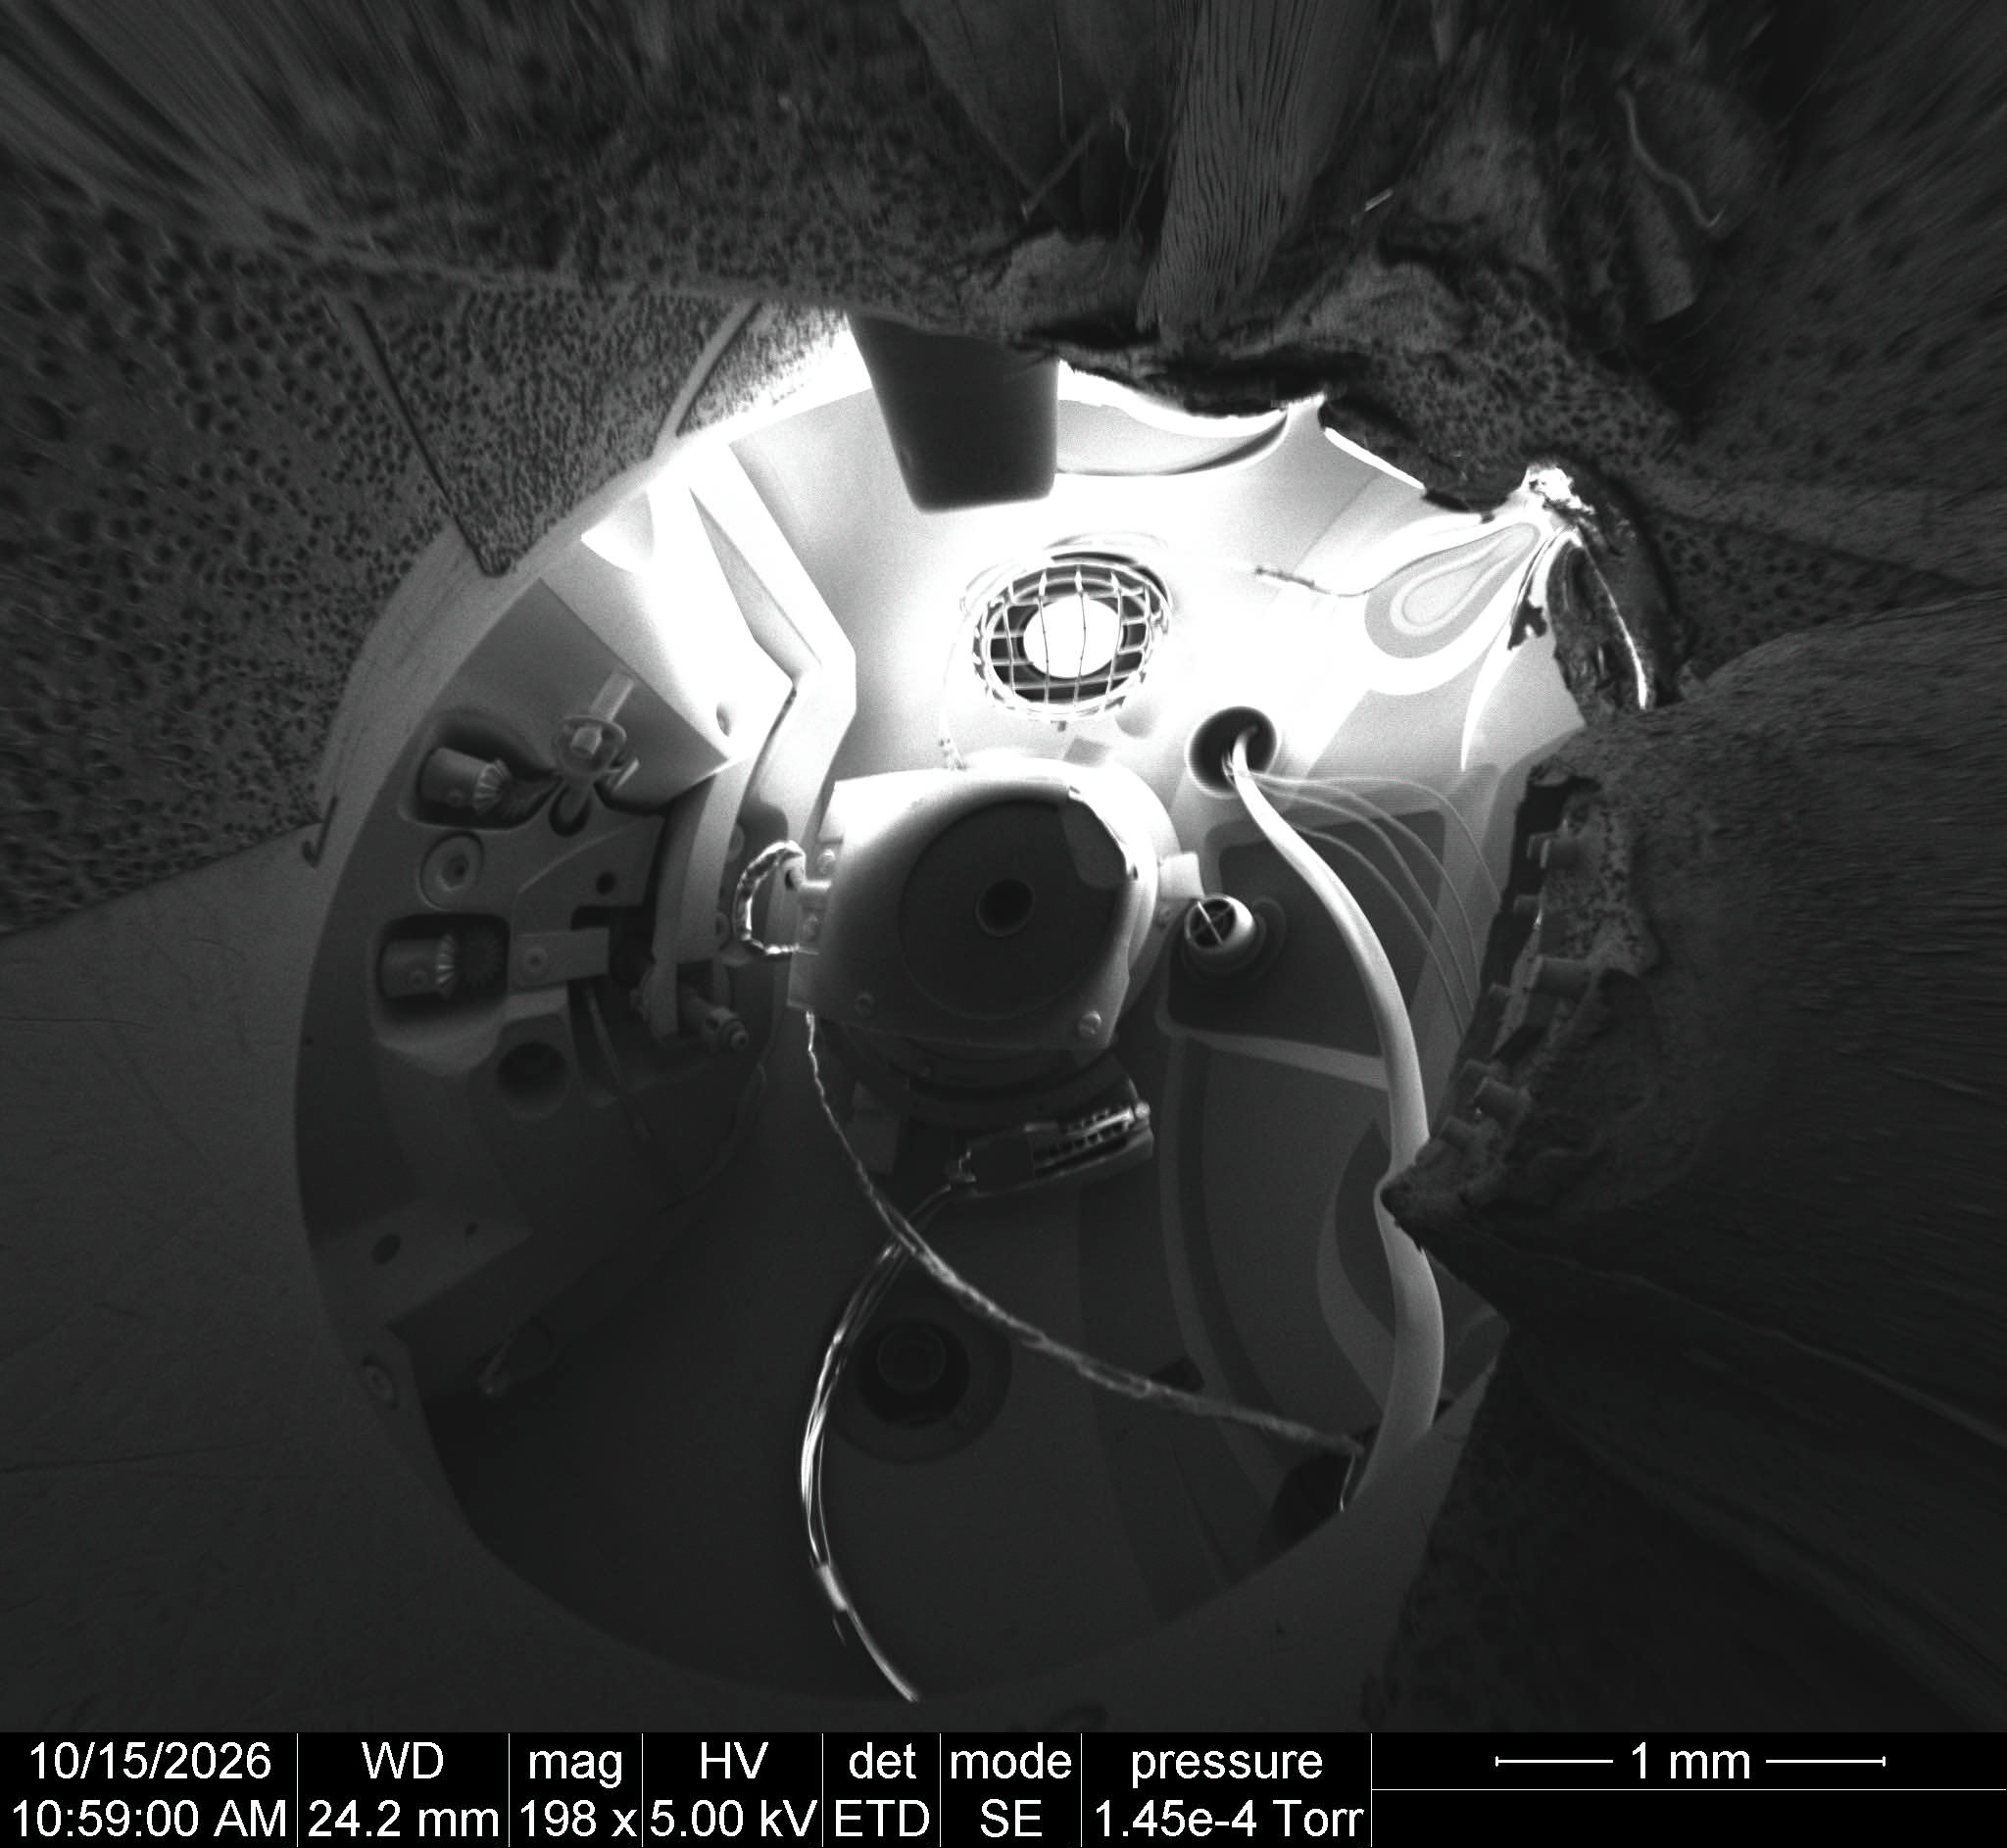
\includegraphics[width=\linewidth]{pp3.jpg}
        \caption {Вид камеры от лица шарика}
        \label{fig:image1}
    \end{minipage}
    \hfill
    \begin{minipage}{0.45\textwidth}
        \centering
        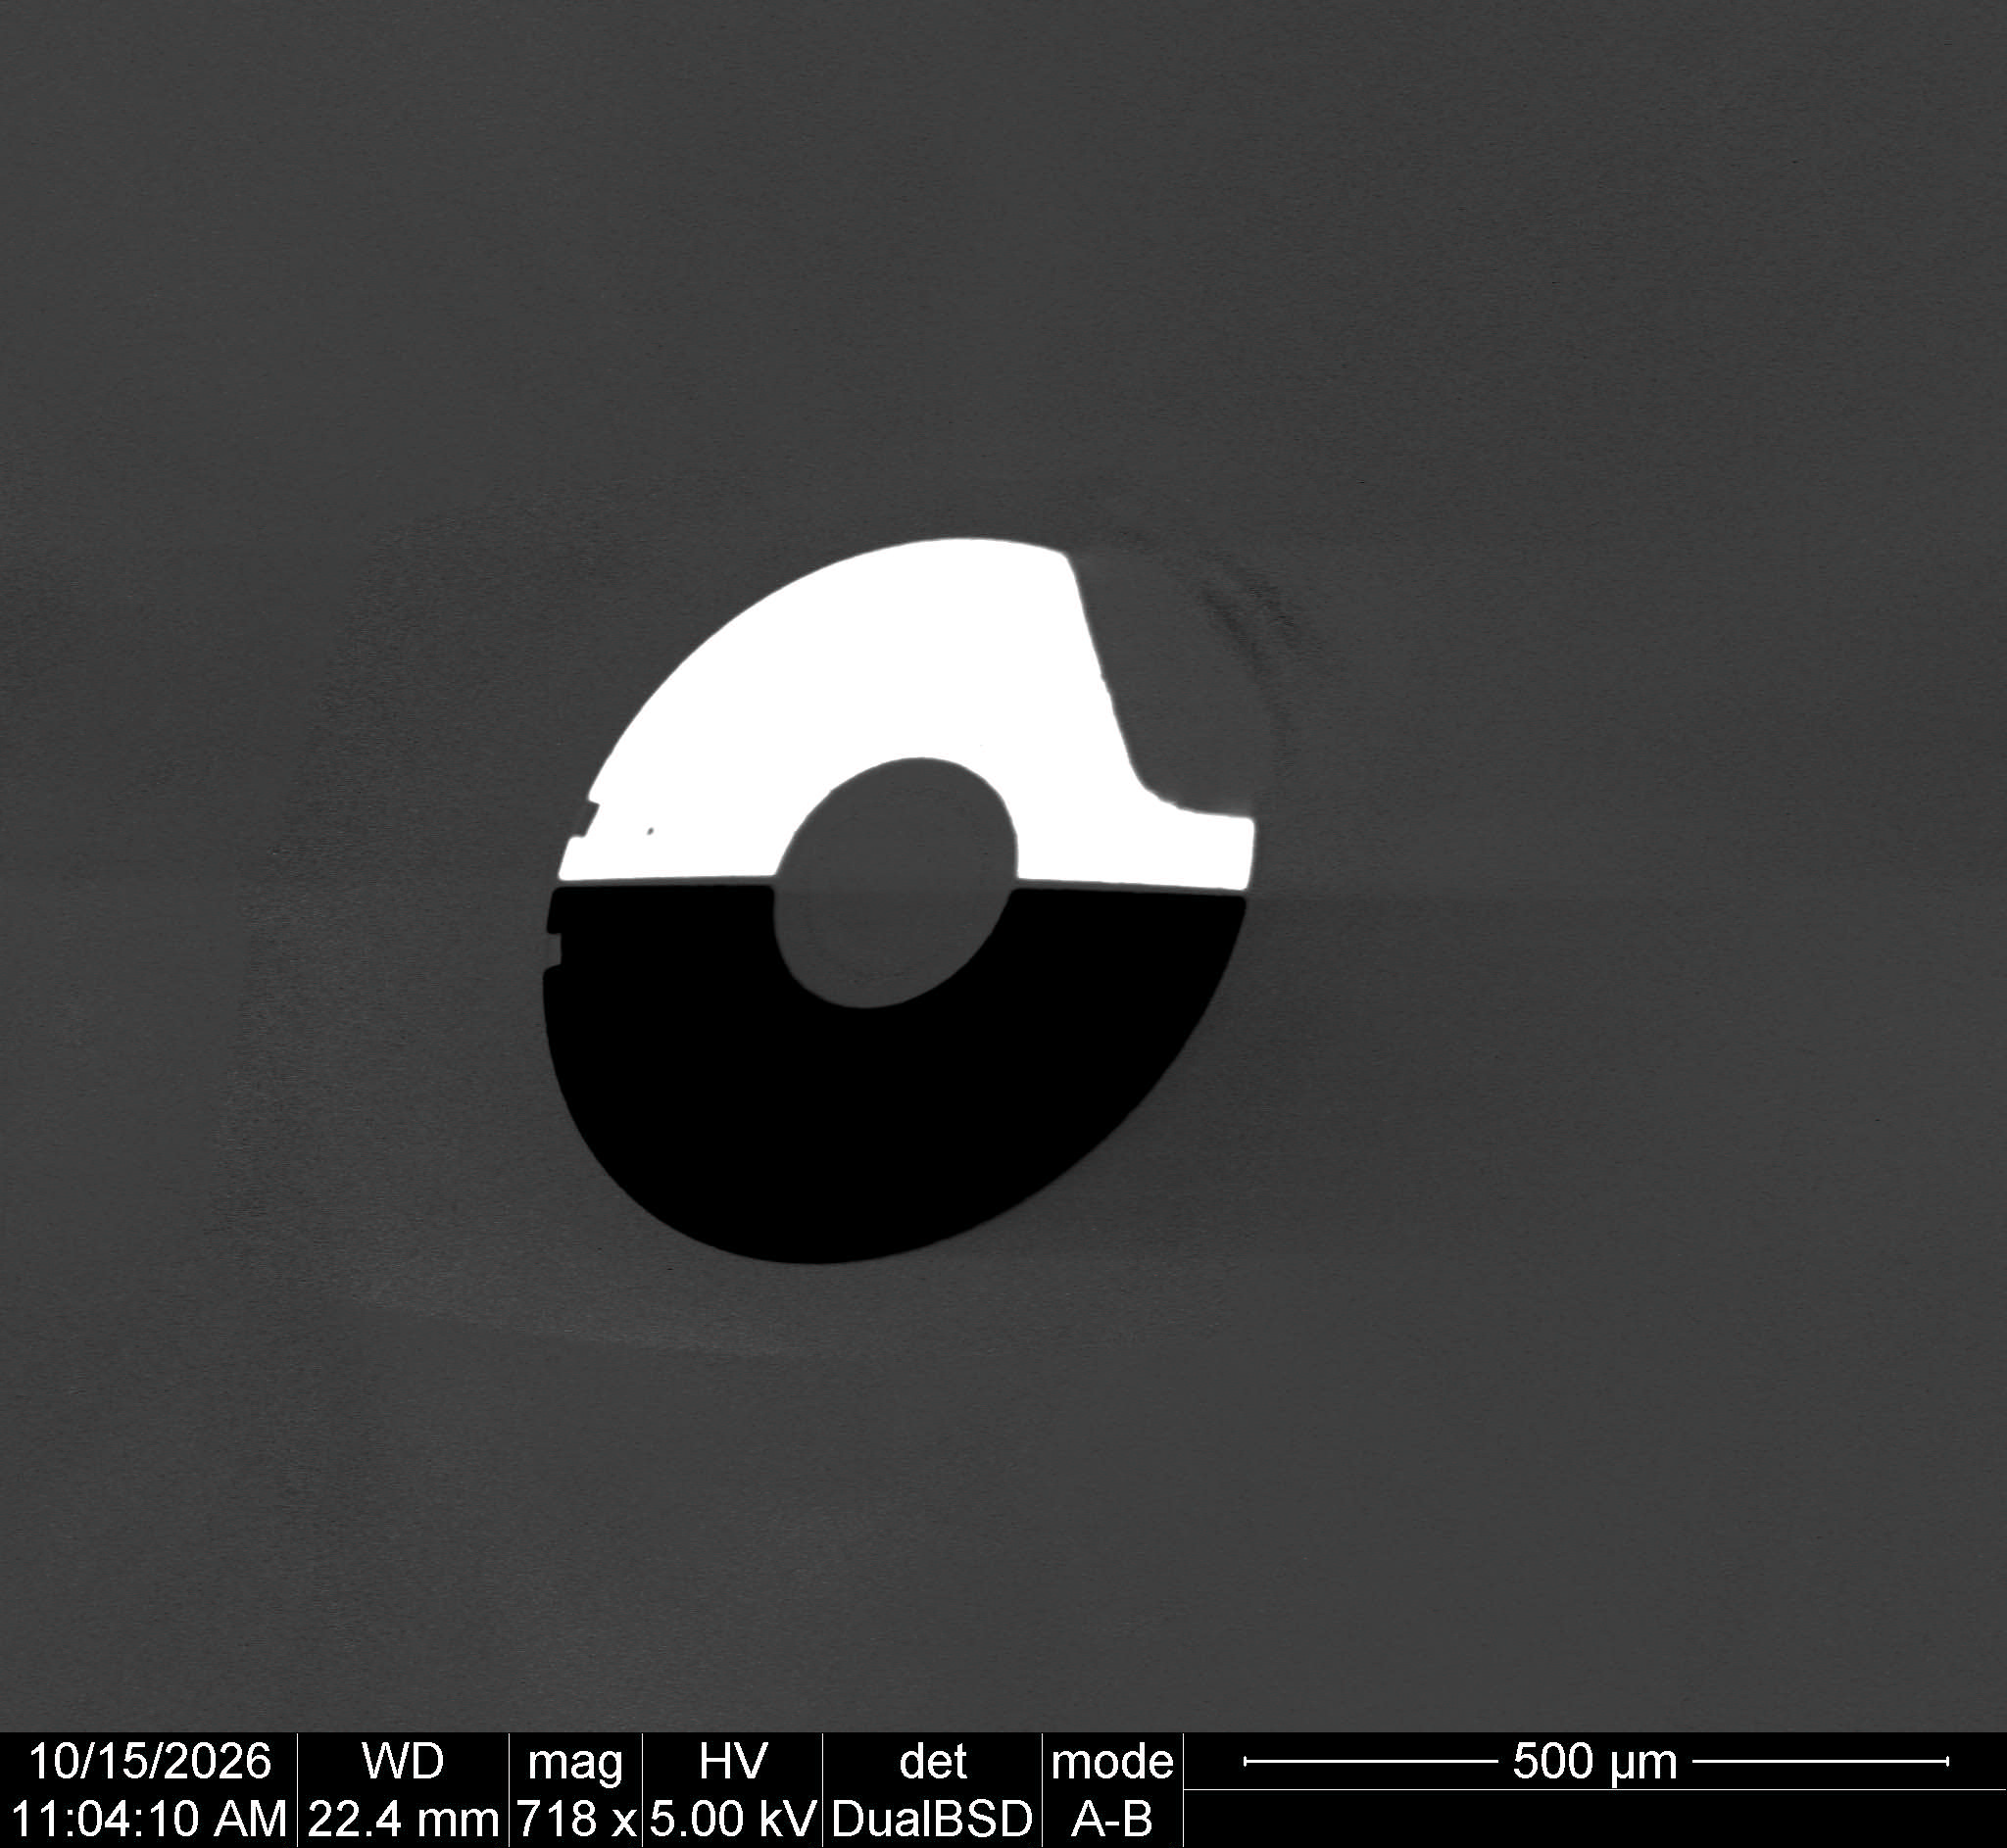
\includegraphics[width=\linewidth]{pp4.jpg}
        \caption{Изображение детектора}
        \label{fig:image2}
    \end{minipage}
\end{figure}


\newpage

\begin{figure}[h]
    \centering
    \begin{minipage}{0.45\textwidth}
        \centering
        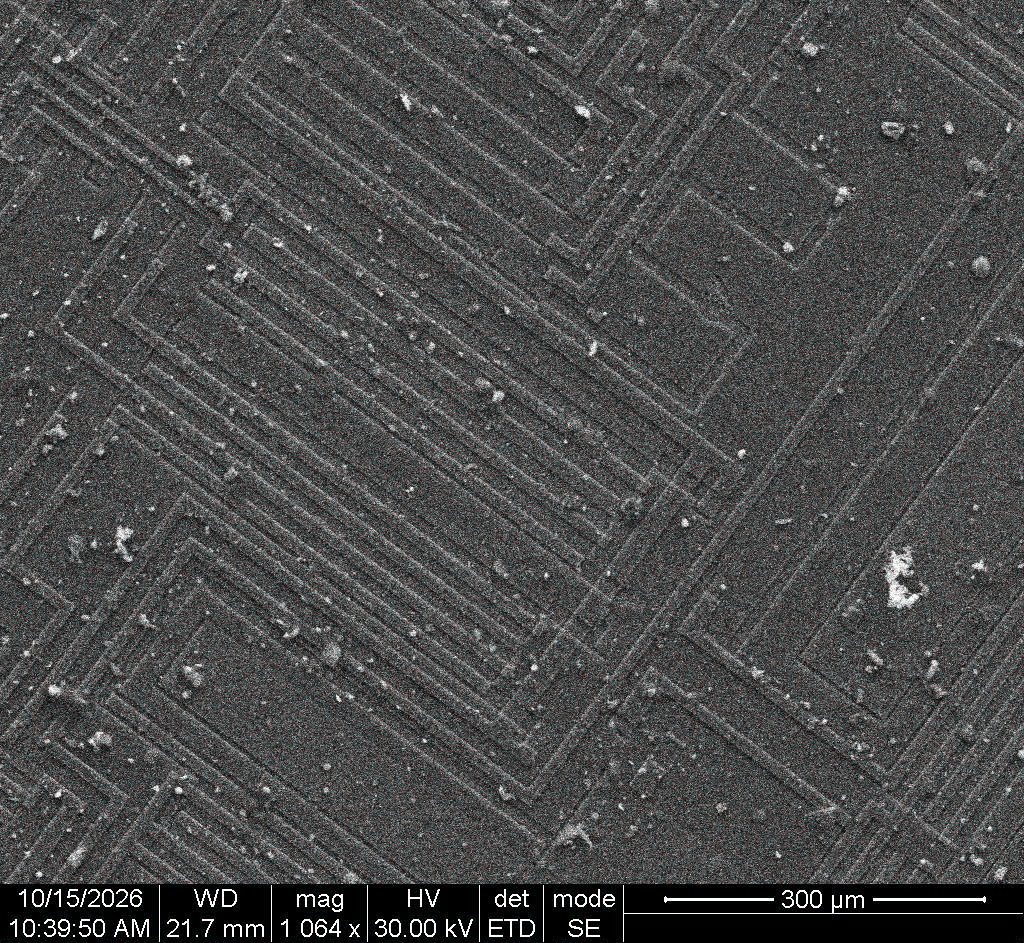
\includegraphics[width=\linewidth]{ppp2.jpg}
        \caption {Изображение микросхемы с малым временем сканирования}
        \label{fig:image1}
    \end{minipage}
    \hfill
    \begin{minipage}{0.45\textwidth}
        \centering
        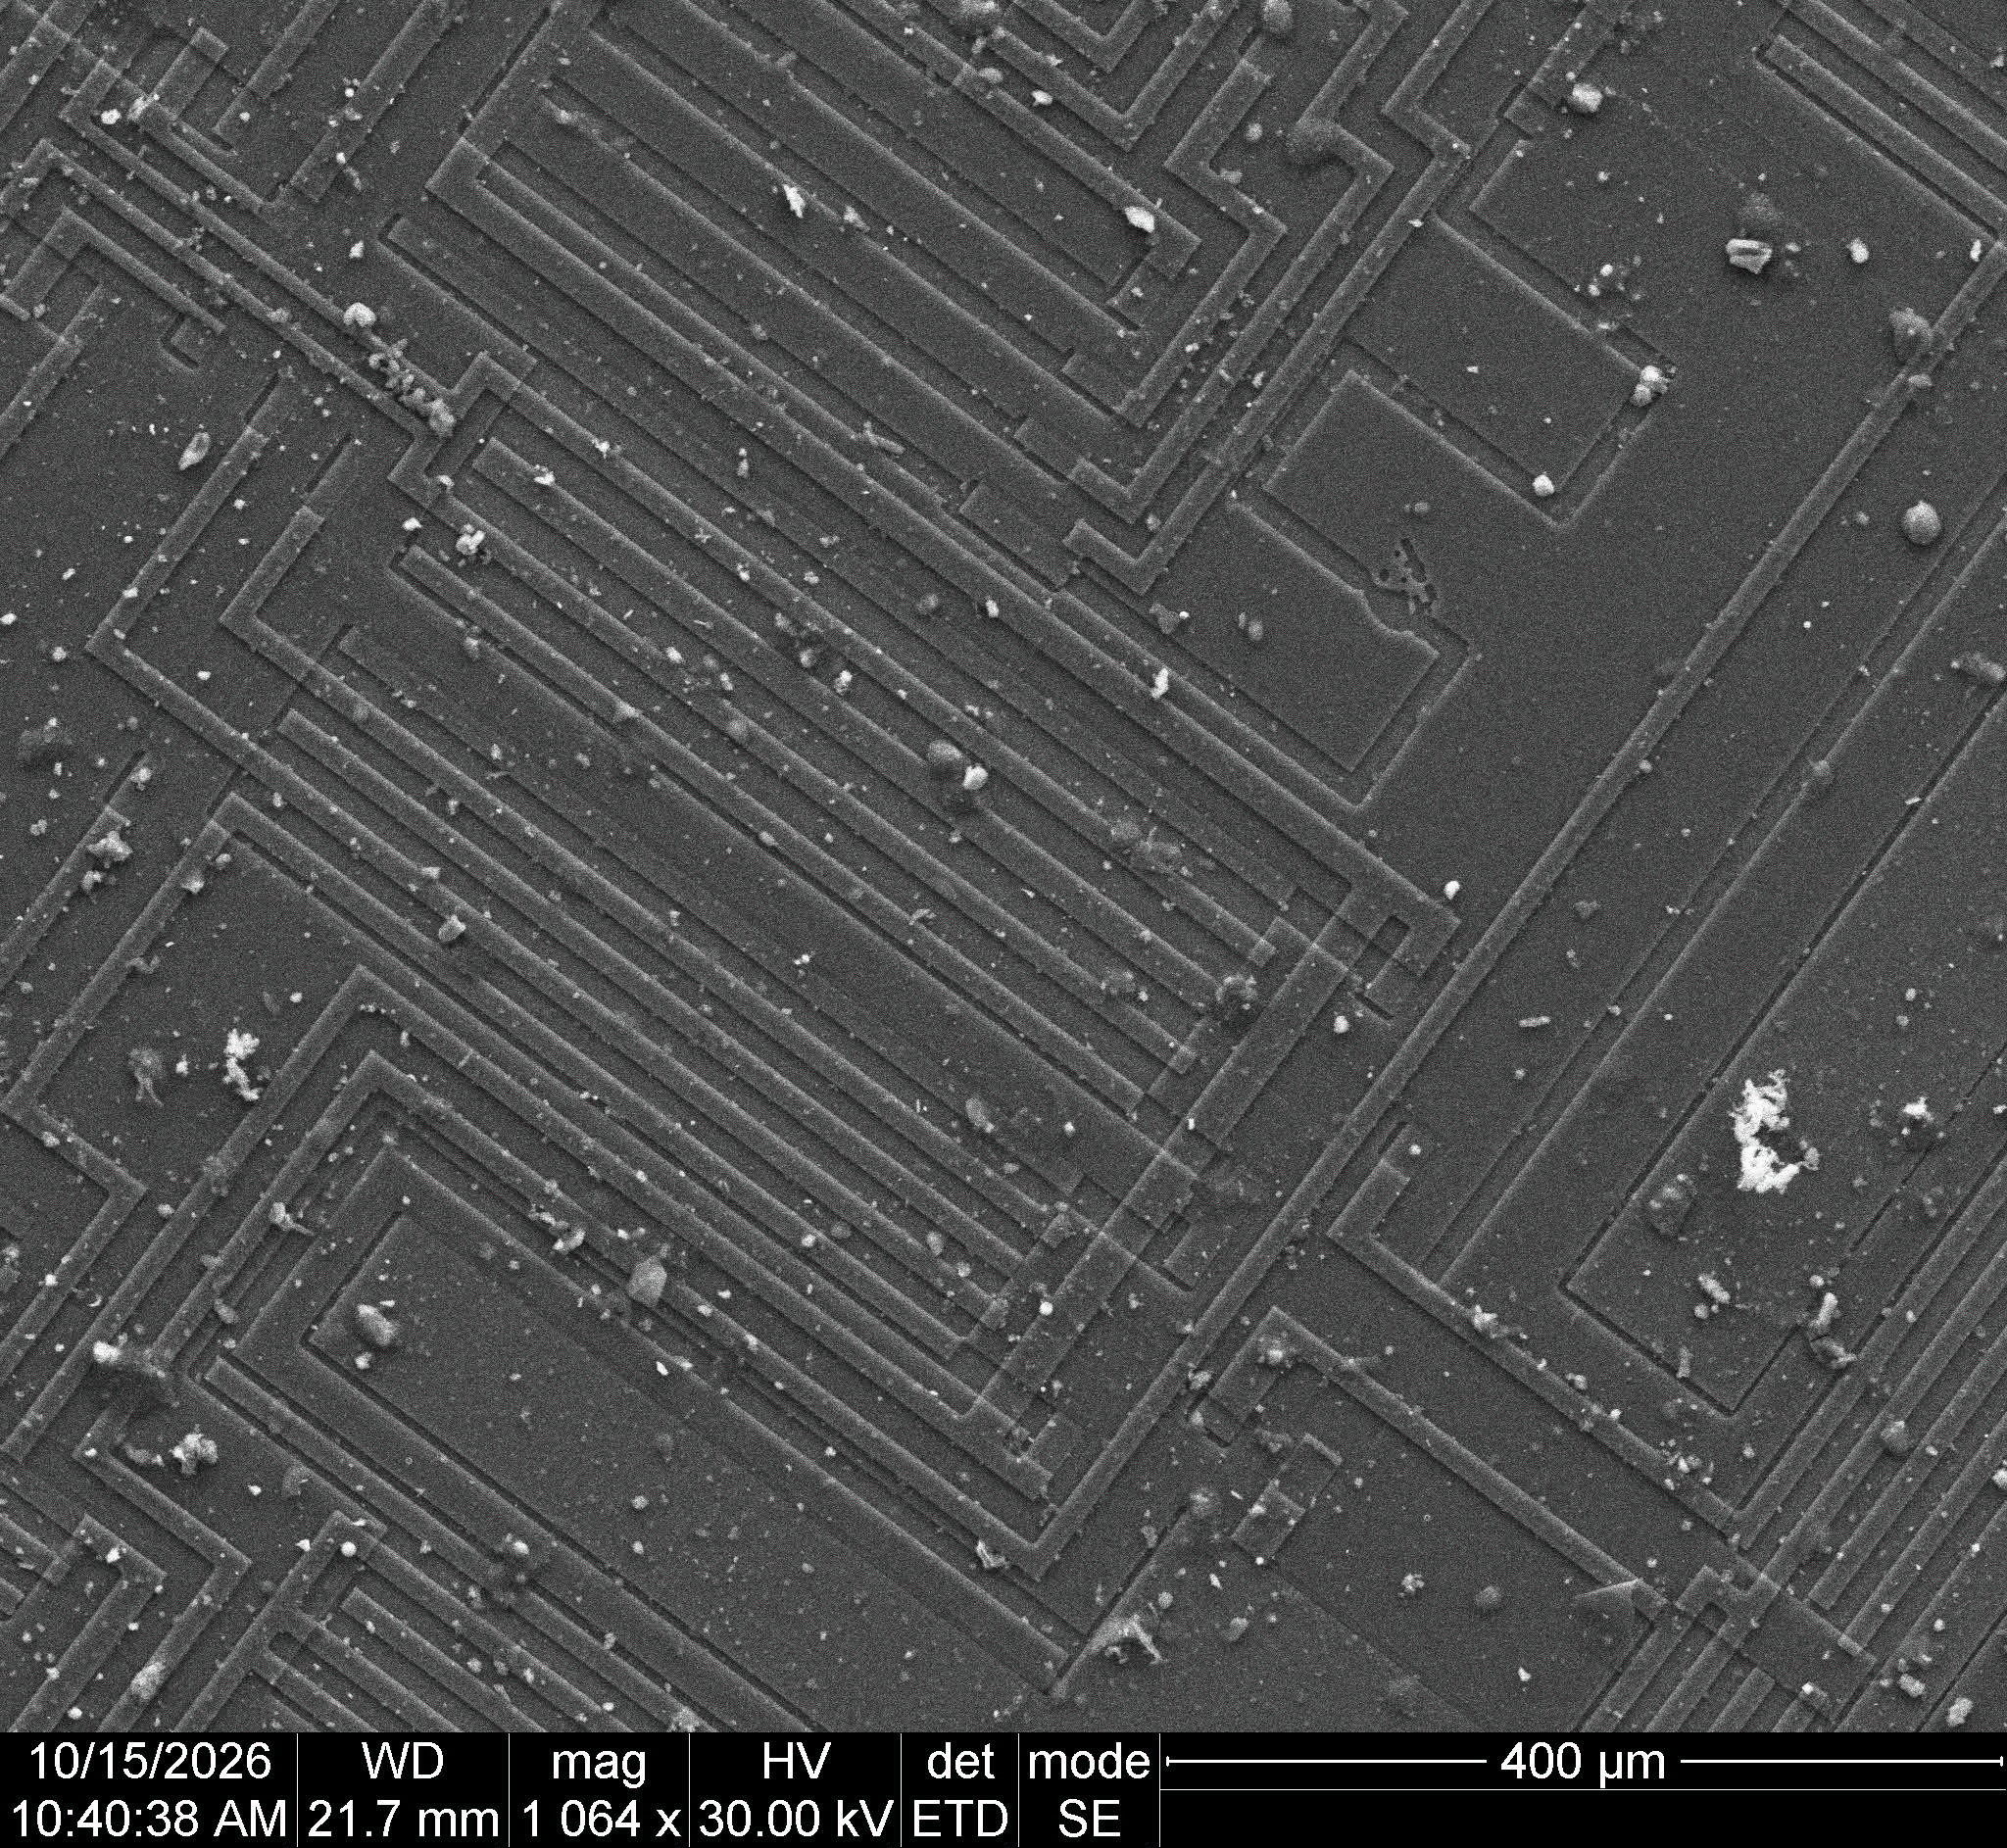
\includegraphics[width=\linewidth]{ppp3.jpg}
        \caption{Изображение микросхемы с большим временем сканирования}
        \label{fig:image2}
    \end{minipage}
\end{figure}

\begin{figure}[h]
    \centering
    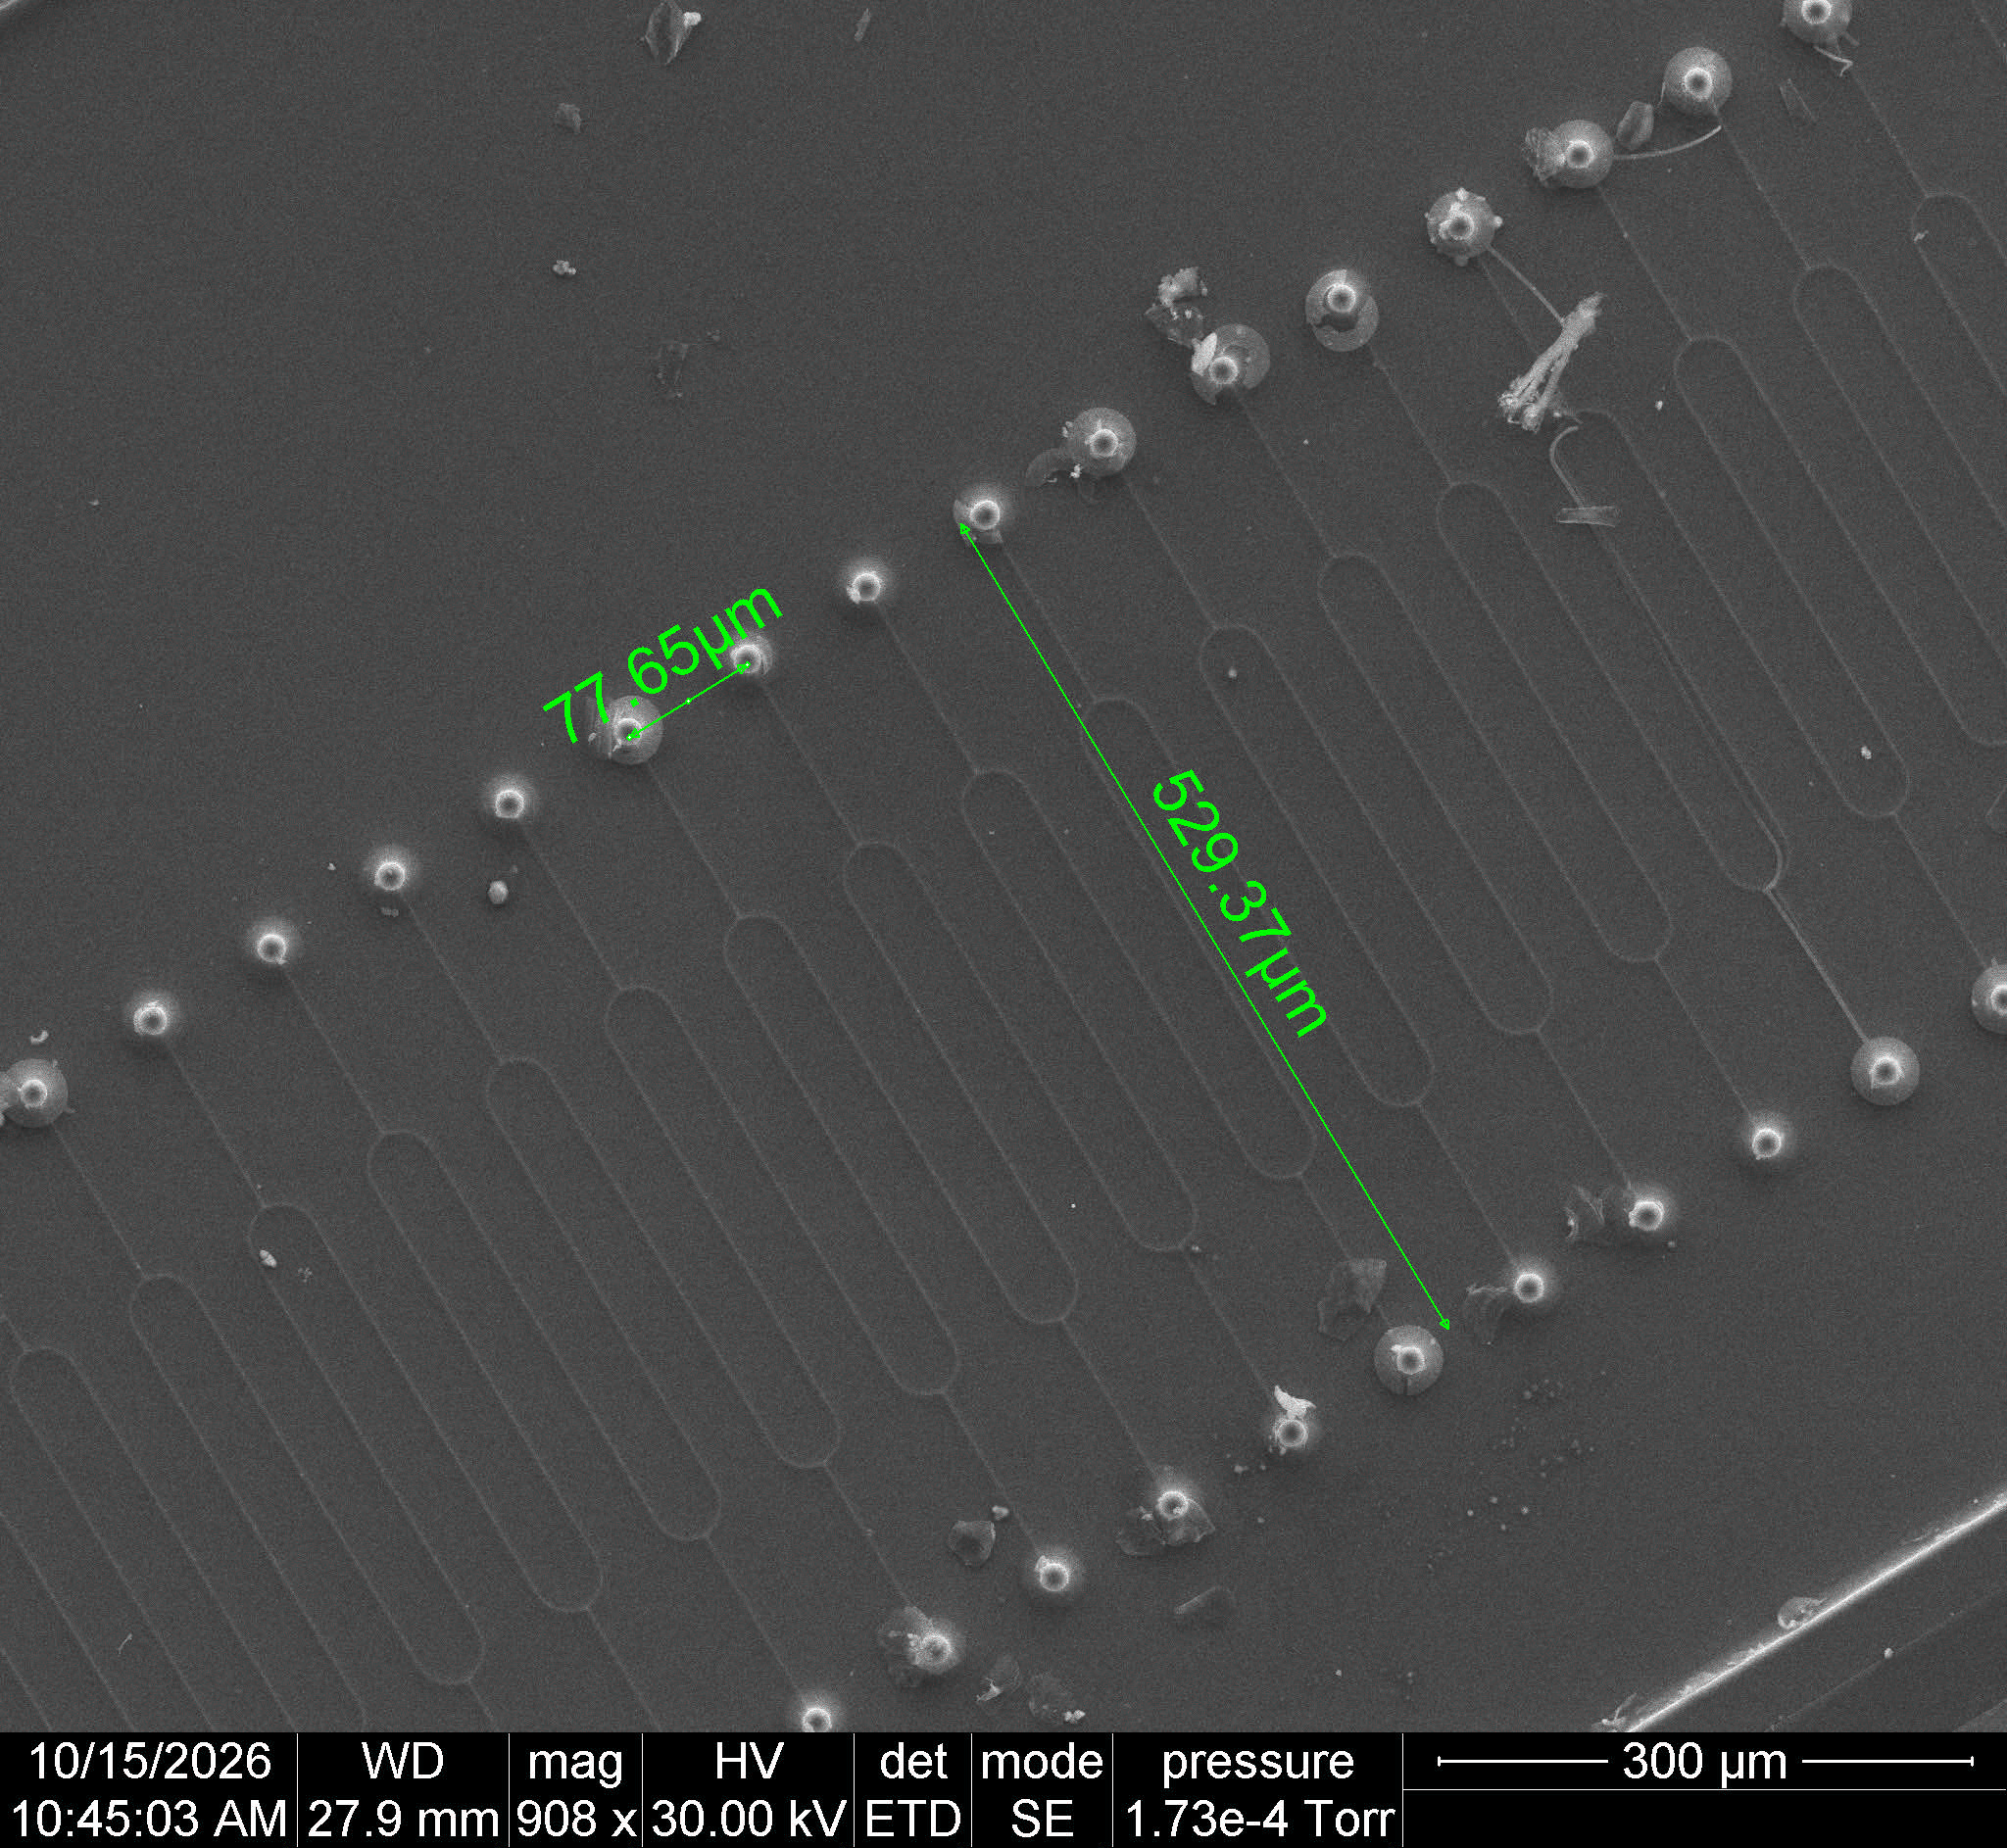
\includegraphics[width=8.5cm]{ppp1.jpg}
    \caption{Изображение дорожек платы (демонстрация возможности измерения расстояния)}
    \label{img_energy_levels}
\end{figure}

\newpage

\begin{figure}[h]
    \centering
    \begin{minipage}{0.45\textwidth}
        \centering
        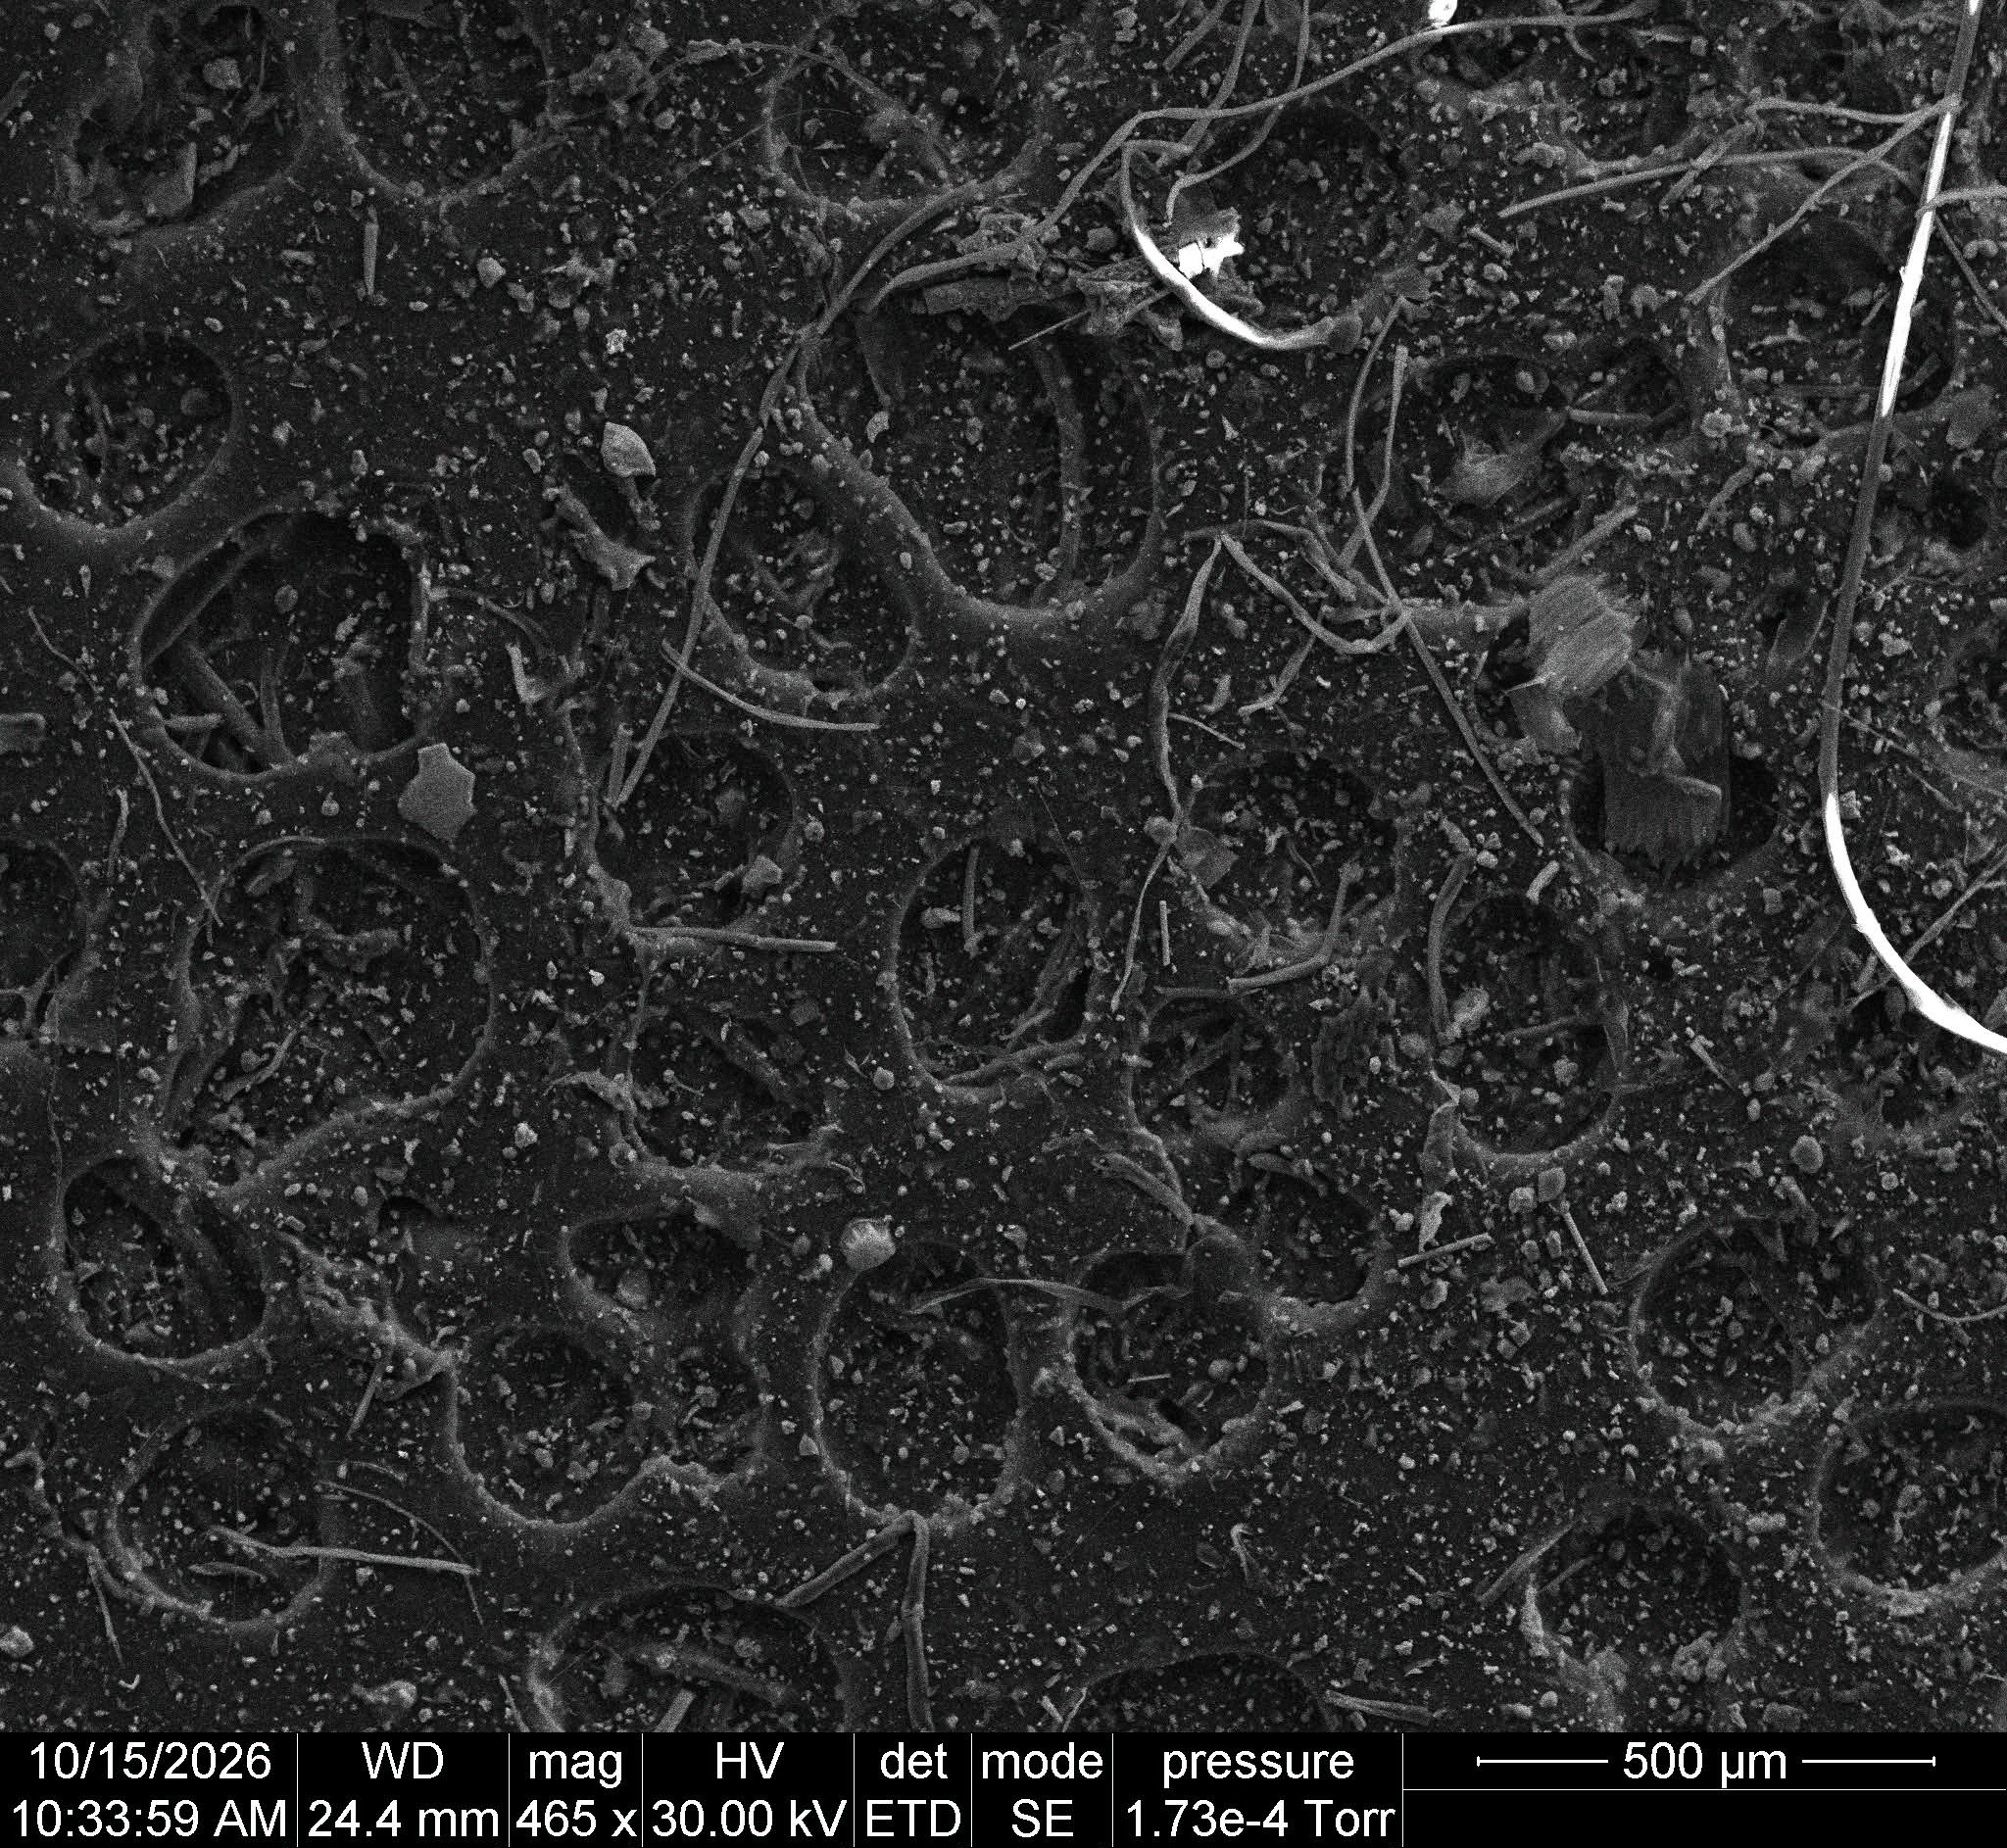
\includegraphics[width=\linewidth]{ppp5.jpg}
        \caption {Возможно структура волокна}
        \label{fig:image1}
    \end{minipage}
    \hfill
    \begin{minipage}{0.45\textwidth}
        \centering
        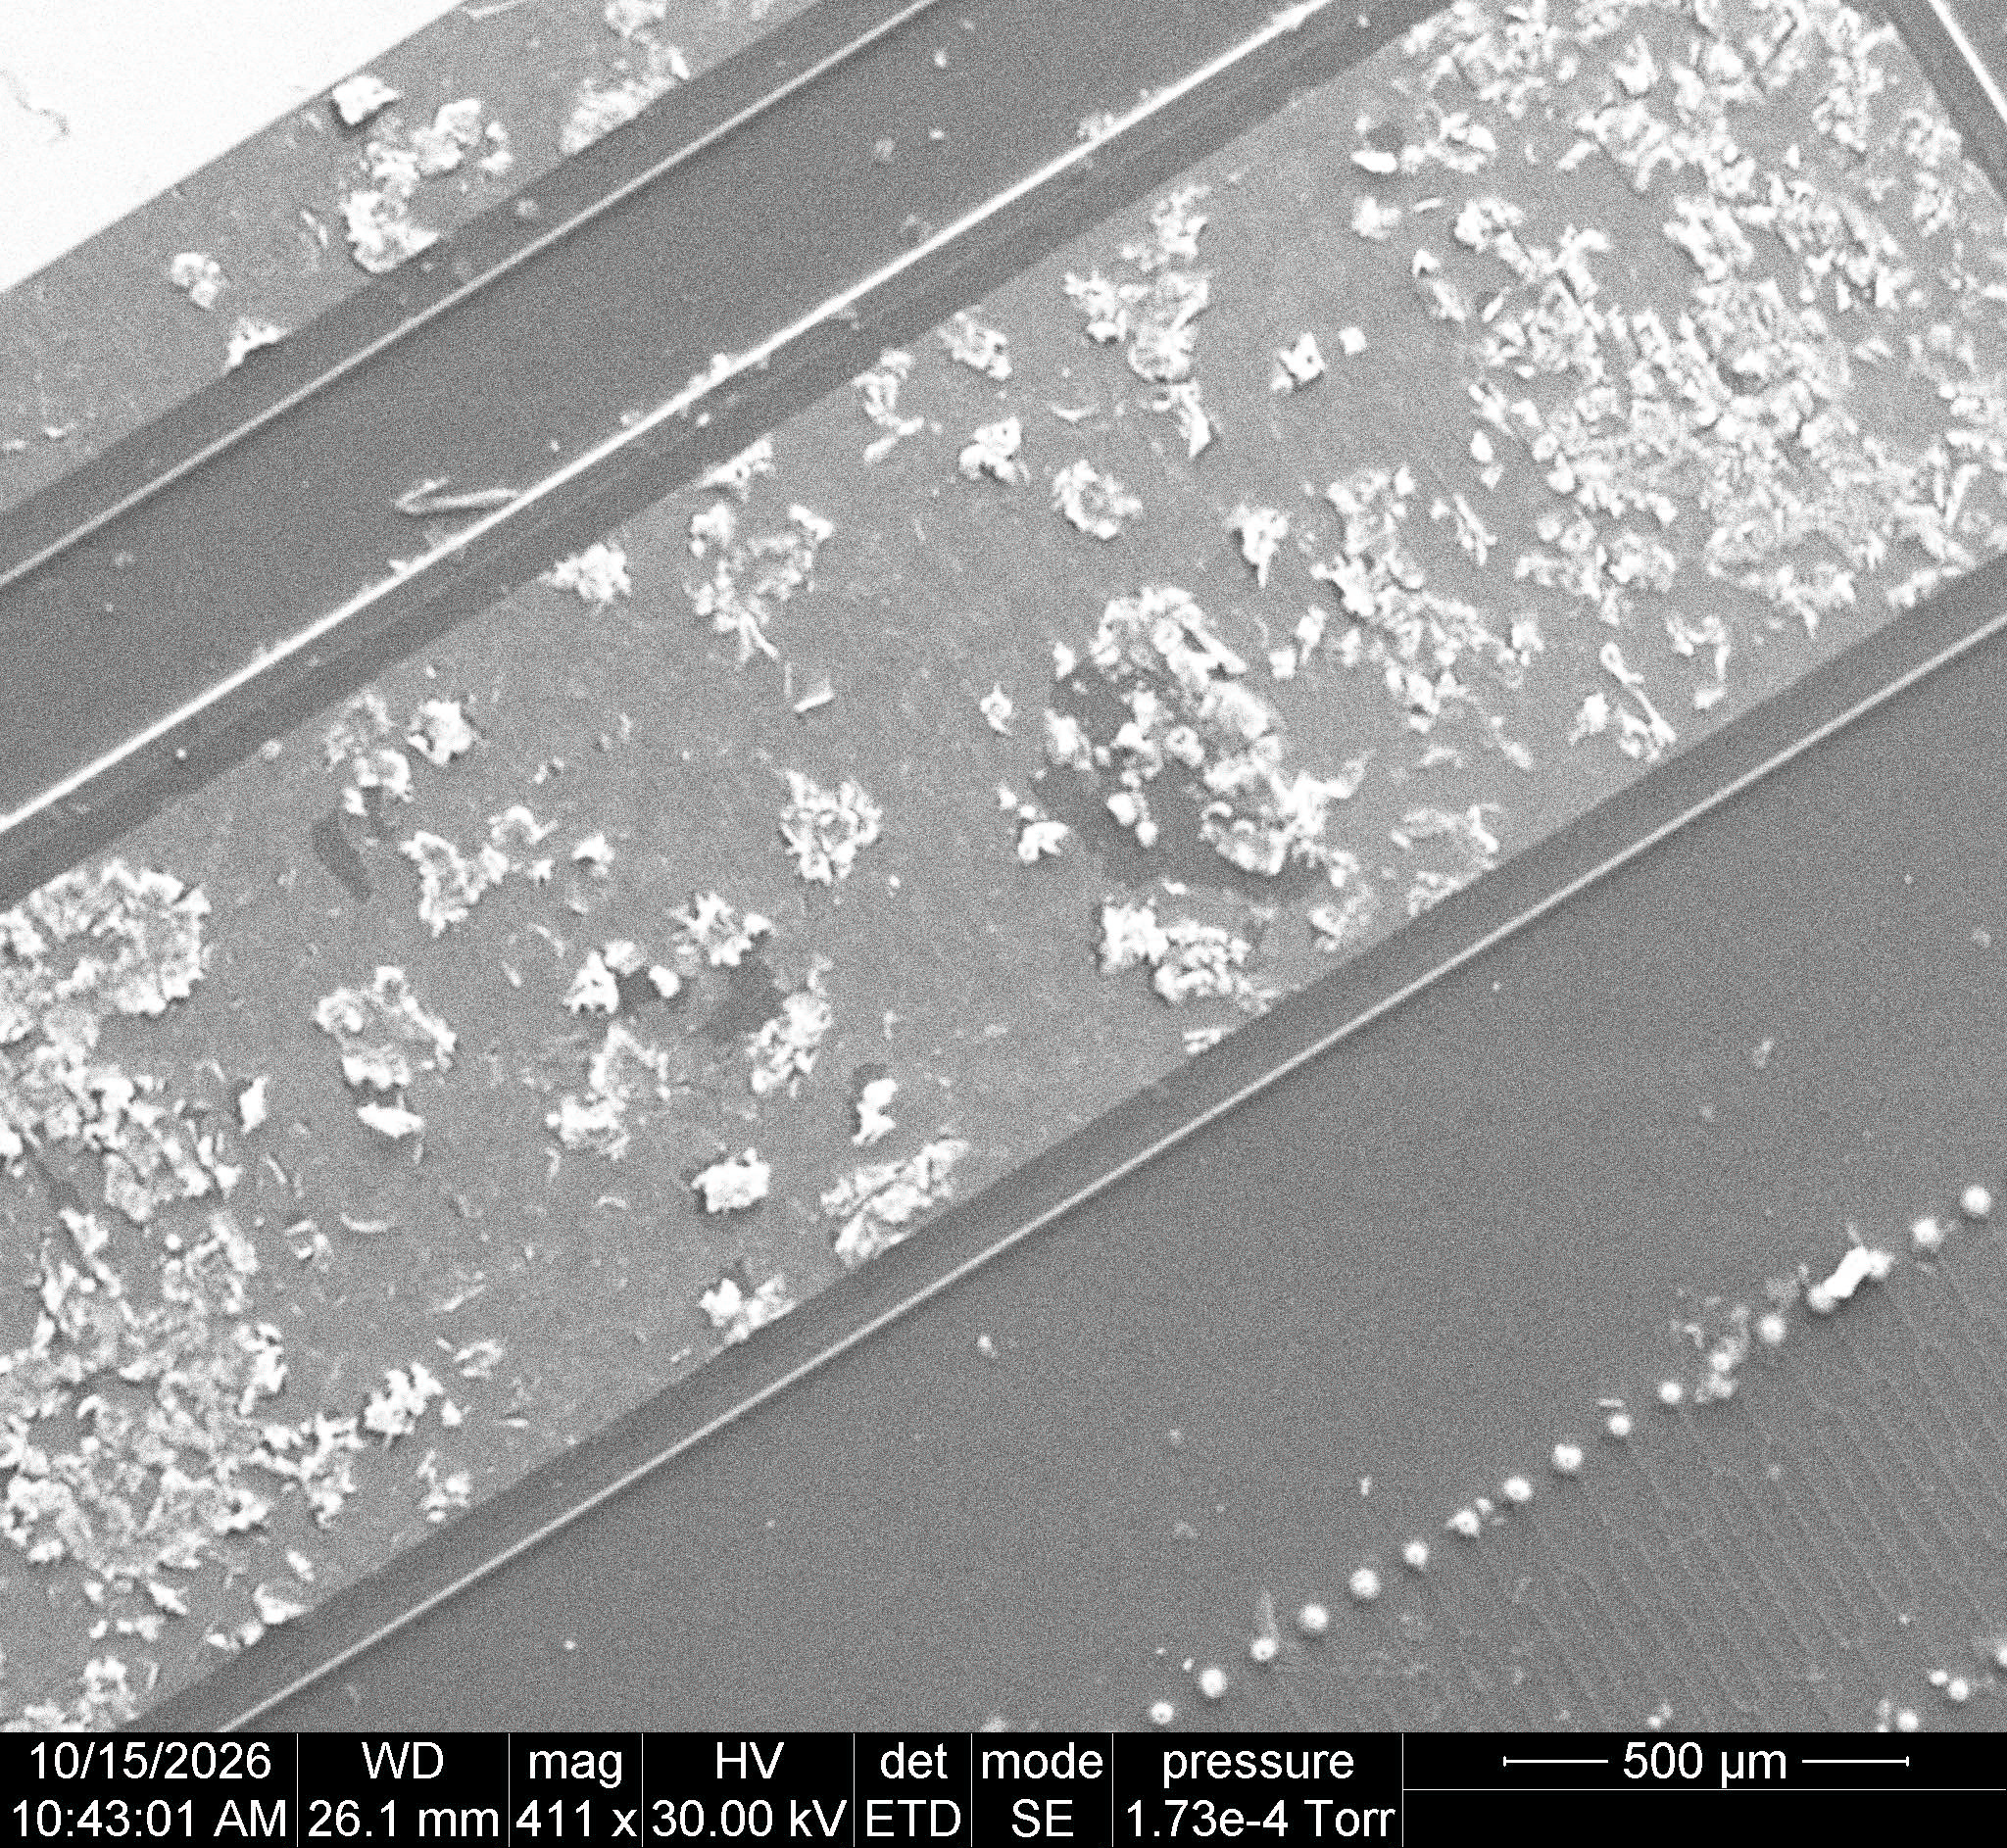
\includegraphics[width=\linewidth]{ppp6.jpg}
        \caption{Изображение коррозии на плате}
        \label{fig:image2}
    \end{minipage}
\end{figure}

\begin{itemize}
  \item Это различие обусловлено временем сканирования (скоростью развертки).
  качество изображения в РЭМ характеризуется соотношением сигнал/шум ($S/N$)
\[
S/N = \frac{n}{\sqrt{n}} = \sqrt{n},
\]
где $n$~--- число вторичных электронов, зарегистрированных в одной точке.
\end{itemize}
\begin{itemize}
    \item На изображении 16 сканирование проводилось быстро. Детектор успел зарегистрировать мало электронов на пиксель, поэтому статистические флуктуации стали сопоставимы с полезным сигналом. Это привело к снижению четкости.
    
    \item На изображении 17 скорость сканирования была снижена. За более долгое время накопления в каждой точке регистрируется значительно больше электронов, что приводит к увеличению $\sqrt{n}$ и, как следствие, к резкому росту соотношения сигнал/шум. Изображение становится детализированным.

    \item На рис 19 продемонстрирована, что огромная глубина резкости РЭМ позволяет одновременно четко видеть и верхние края ячеек, и их глубокое дно.
\end{itemize} 

\subsection{Численный эксперимент}

В численном эксперименте мы снимали значения силы тока и погрешность с поверхности и с дырки цилиндра при различных напряжениях.

Результаты приведены в таблице


Эффективный коэффициент электронной эмиссии вычислялся как:

\[
\delta_{\mathrm{eff}} = \frac{I_{\mathrm{hole}} - I_{\mathrm{surf}}}{I_{\mathrm{hole}}} = 1 - \frac{I_{\mathrm{surf}}}{I_{\mathrm{hole}}}.
\]
\newpage

\begin{figure}[h]
    \centering
    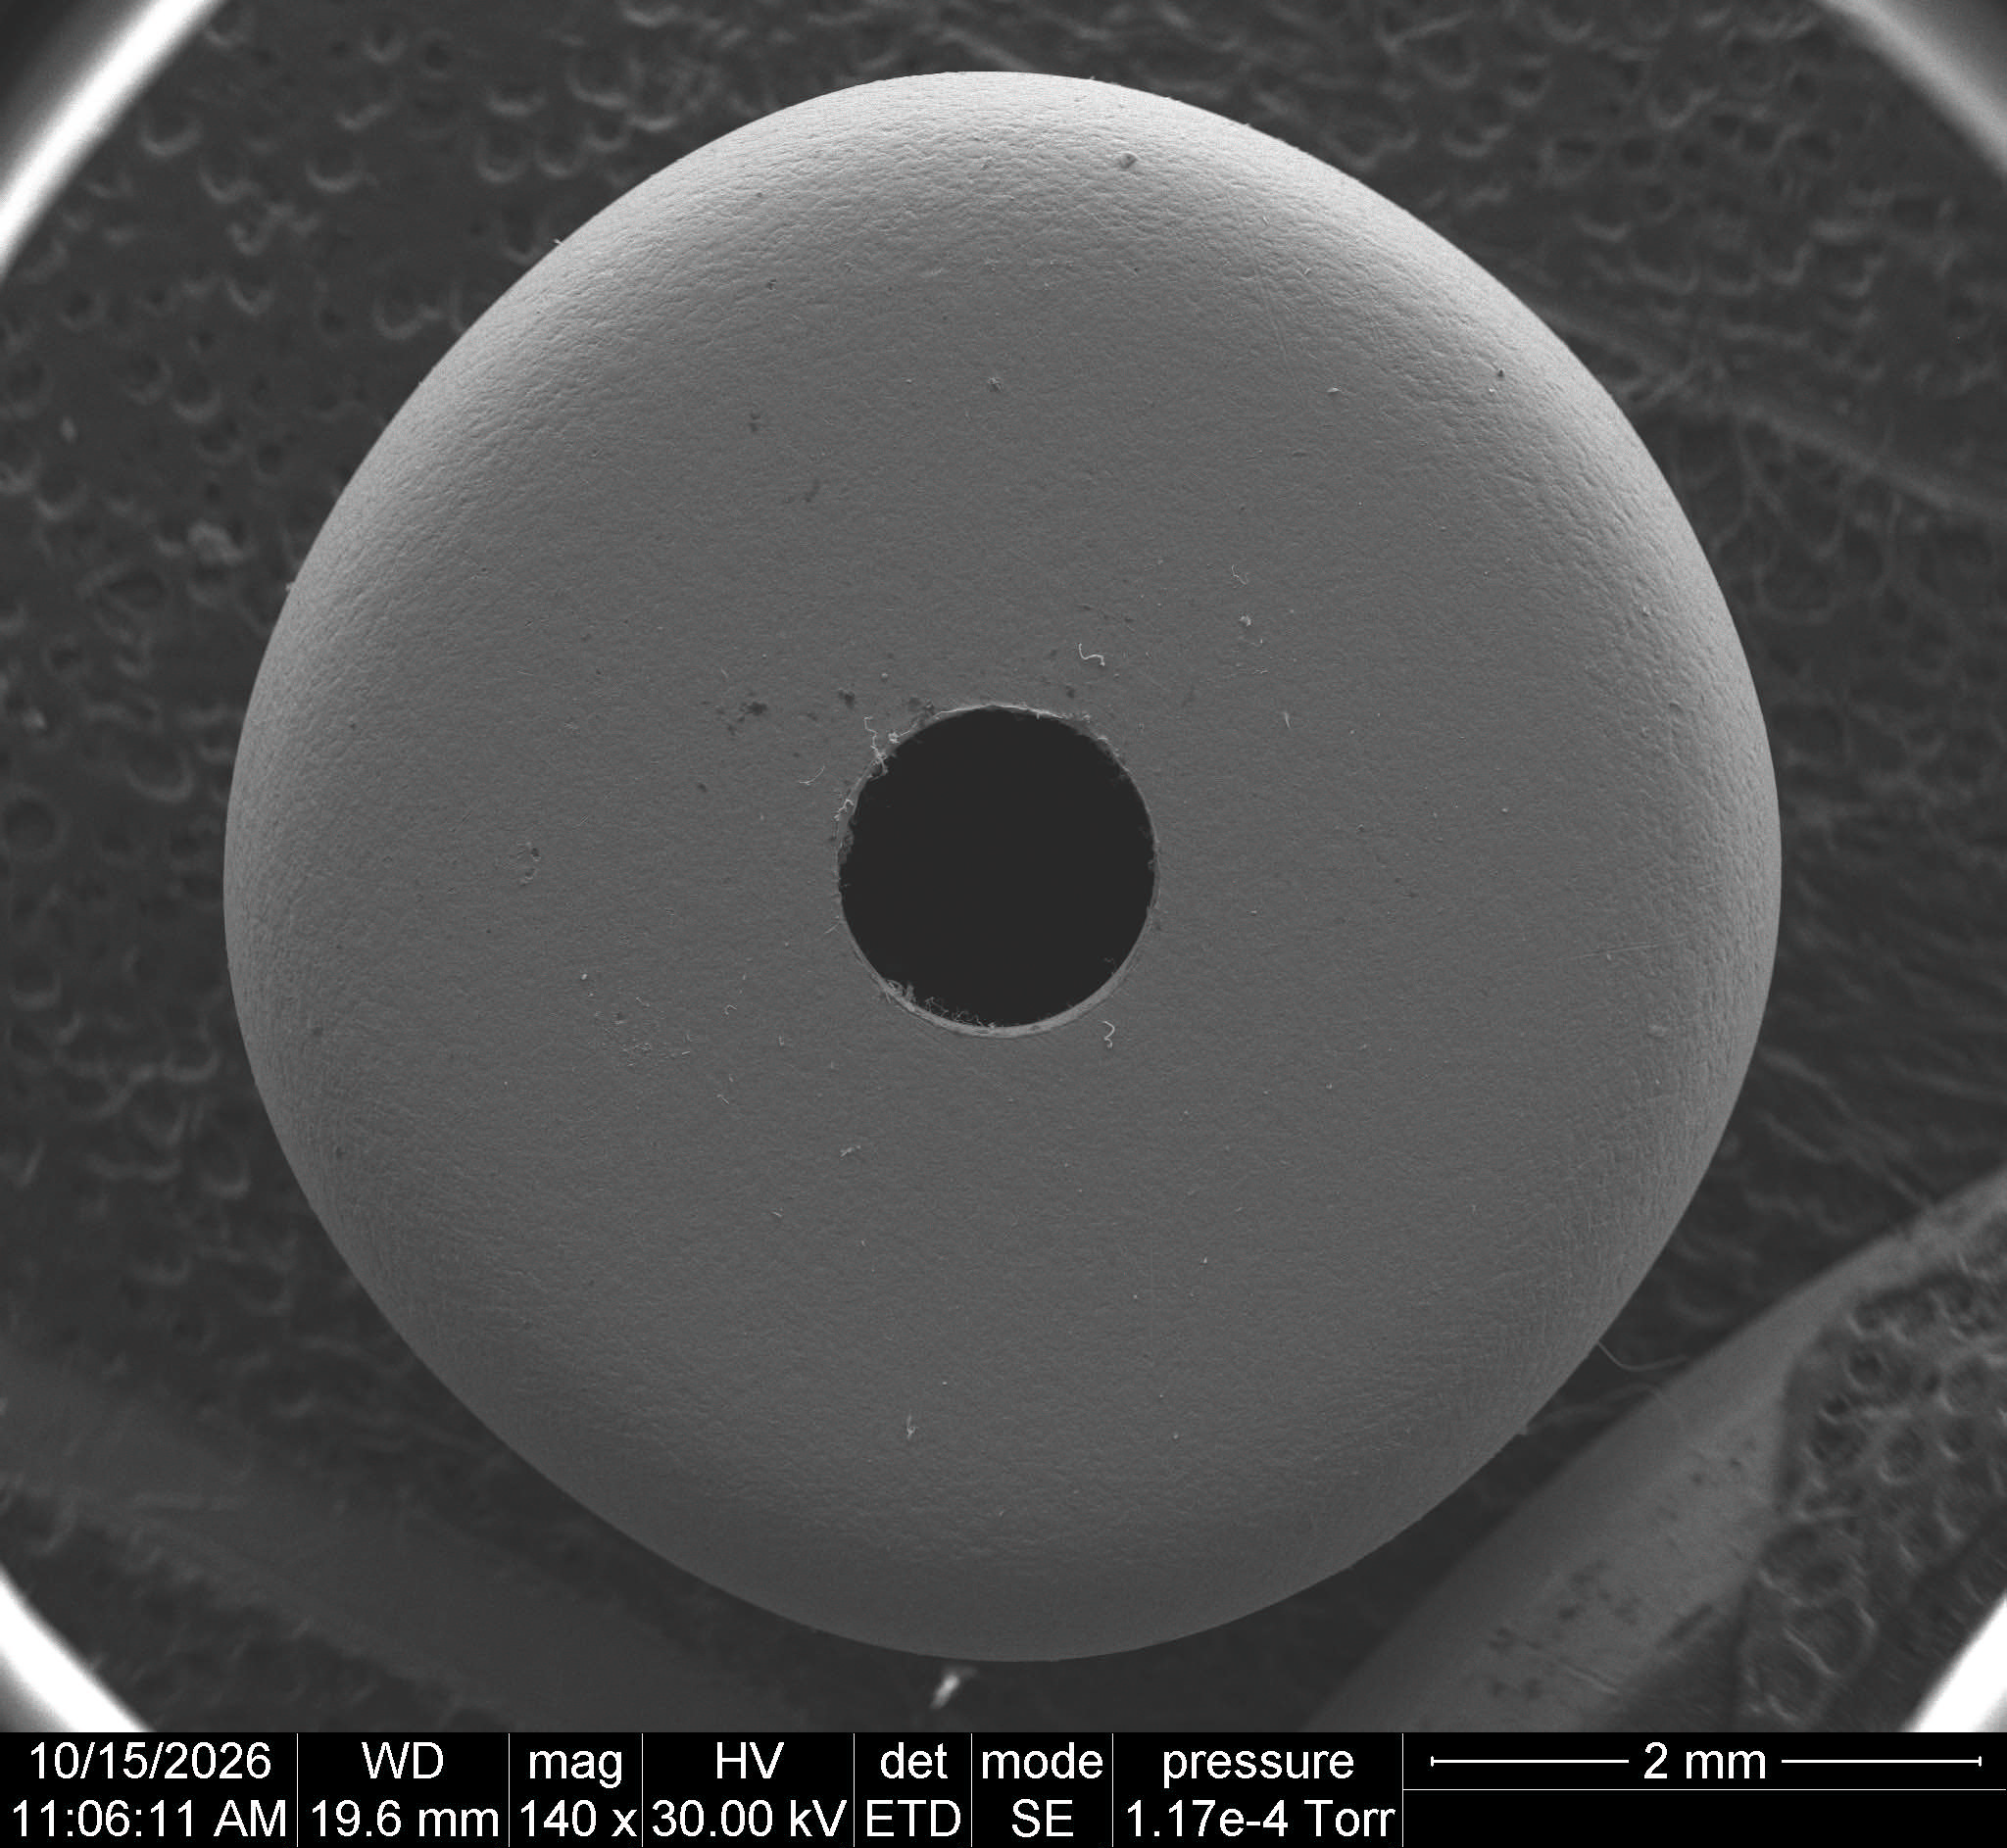
\includegraphics[width=8.5cm]{ppp4.jpg}
    \caption{Цилиндр}
    \label{img_energy_levels}
\end{figure}

\begin{table}[h]
\centering
\caption{Зависимость токов от напряжения}
\label{tab:currents_voltage}
\begin{tabular}{|c|c|c|c|}
\hline
$U$, кВ & $I_{\text{hole}}$, пкА & $I_{\text{surf}}$, пкА & $\delta_{\text{eff}}$ \\
\hline
30{,}00 & 88{,}00 & 64{,}00 & 0{,}27 \\
25{,}00 & 70{,}00 & 51{,}00 & 0{,}27 \\
20{,}00 & 57{,}00 & 41{,}00 & 0{,}28 \\
17{,}00 & 50{,}00 & 36{,}00 & 0{,}28 \\
15{,}00 & 43{,}00 & 31{,}00 & 0{,}28 \\
12{,}50 & 48{,}00 & 35{,}00 & 0{,}27 \\
10{,}00 & 40{,}00 & 30{,}00 & 0{,}25 \\
5{,}00  & 32{,}00 & 24{,}00 & 0{,}25 \\
2{,}00  & 30{,}00 & 25{,}00 & 0{,}17 \\
1{,}00  & 37{,}00 & 31{,}00 & 0{,}16 \\
0{,}50  & 5{,}00  & 5{,}00  & 0{,}00 \\
\hline
\end{tabular}
\end{table}

Для функции двух независимых величин приборная составляющая погрешности определяется через частные производные:
\[
\sigma_{\delta,\mathrm{pr}} = \sqrt{ \left( \frac{\partial \delta}{\partial I_{\mathrm{surf}}} \Delta I_{\mathrm{surf}} \right)^2 + \left( \frac{\partial \delta}{\partial I_{\mathrm{hole}}} \Delta I_{\mathrm{hole}} \right)^2 }.
\]

Здесь
\[
\frac{\partial \delta}{\partial I_{\mathrm{surf}}} = -\frac{1}{I_{\mathrm{hole}}}, \qquad \frac{\partial \delta}{\partial I_{\mathrm{hole}}} = \frac{I_{\mathrm{surf}}}{I_{\mathrm{hole}}^2}.
\]

Поэтому
\[
\sigma_{\delta,\mathrm{pr}} = \sqrt{ \left( \frac{\Delta I_{\mathrm{surf}}}{I_{\mathrm{hole}}} \right)^2 + \left( \frac{I_{\mathrm{surf}} \Delta I_{\mathrm{hole}}}{I_{\mathrm{hole}}^2} \right)^2 }.
\]

Например, для второй точки
\[
I_{\mathrm{hole}} = 37{,}0~\text{нА}, \qquad I_{\mathrm{surf}} = 31{,}0~\text{нА},\qquad \Rightarrow \sigma_{\delta,\mathrm{pr}} = 3,5 * 10^{-5},\qquad \text{т.е очень мало по сравнению с эксп данными}
\]

\newpage

Для описания диапозона использовалась функция: 

\[
\delta_{\mathrm{fit}}(U_0) = \delta_m \left( \frac{U_0}{U_m} \right)^s \exp\left[ s \left( 1 - \frac{U_0}{U_m} \right) \right].
\]

\[
r_i = \delta_i - \delta_{\mathrm{fit}}(U_i).
\]

\[
\sigma_{\mathrm{res}} = \sqrt{\frac{\sum_{i=1}^{N} r_i^2}{N - m}},
\]

\textbf{Стьюдент}

\[
t_{0.975,\,9} = 2{,}262.
\]

\[
\Delta\delta_{\mathrm{res}} = t_{0.975,\,9} \, \sigma_{\mathrm{res}} \approx 0{,}0210.
\]

В итоге погрешность получилась: 

\[
\Delta\delta_i = \sqrt{ (\Delta\delta_{\mathrm{res}})^2 + (\sigma_{\delta,\mathrm{pr},i})^2 } \approx 0,02.
\]

\begin{figure}[h]
    \centering
    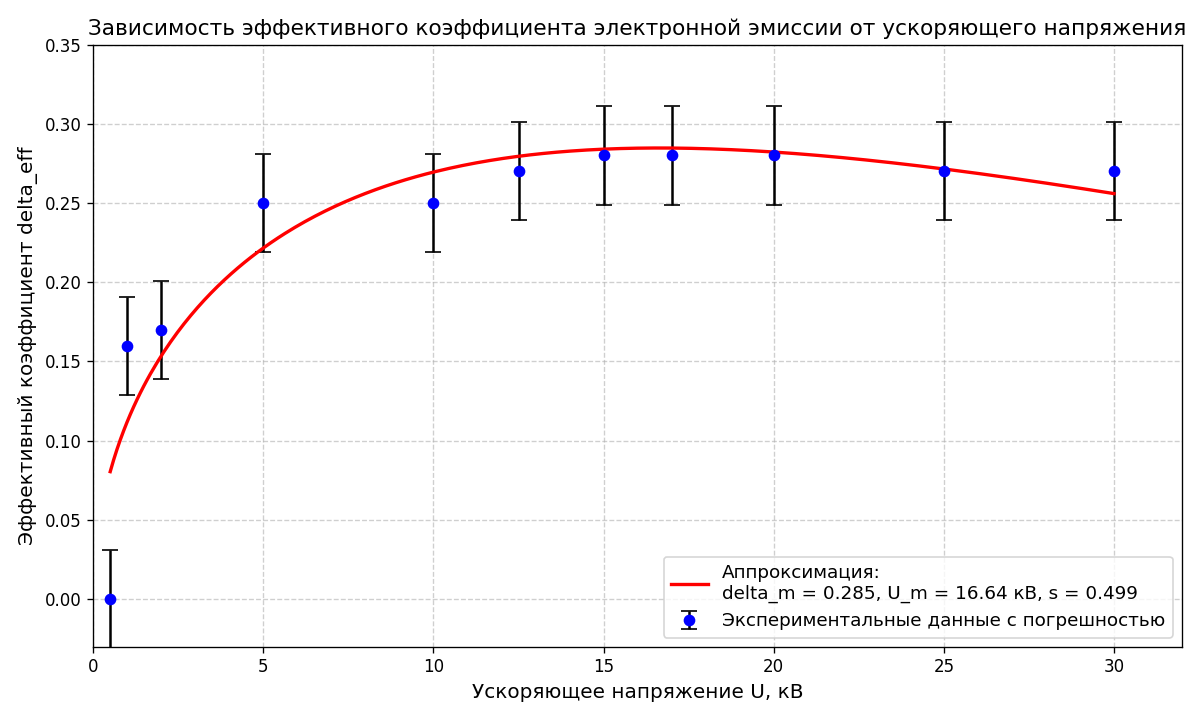
\includegraphics[width=15cm]{F1.png}
    % \caption{Цилиндр}
    \label{img_energy_levels}
\end{figure}

\newpage

\section{Вывод}

\begin{enumerate}
  \item Ознакомились с физическими принципами функционирования РЭМ
  \item Получили множество изображений разных образцов при разных режимах работы микроскопа
  \item Изучили физические принципы формирования изображения в РЭМ (на примере пенопластового шарика более наглядно видно)
  \item Провели численный эксперимент и построили график зависимости эффективного коэффициента электронной эмиссии от ускоряющего напряжения
  \item Посчитали погрешность построения графика $\approx 0.02$ 
\end{enumerate}

\end{document}